\chapter{Image formation} \label{ch:image_formation}

% Wat meten we: CT, PET, SPECT (attenuated projection)
%--------------
% planar
%--------
%
% 2D Tomography
%-----------
%
% Fully 3D Tomography
%-----------
%
% Mathematical model of the acquisition process
%-----------
\begin{figure}[tb]
\centering
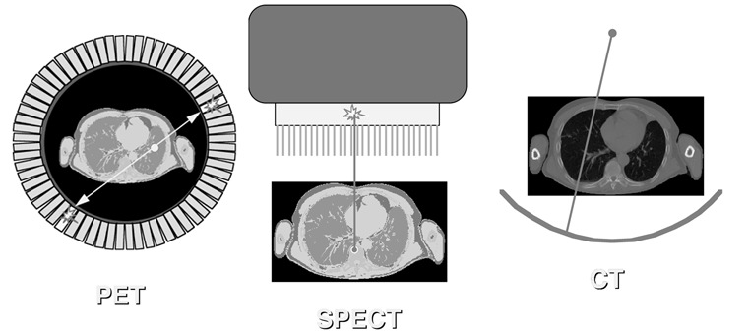
\includegraphics[width=0.75\textwidth]{figs/fig_spect_pet_ct.pdf}
\caption{\label{fig:spect_pet_ct_bis} \emph{Information acquired along lines
in the PET camera, the gamma camera and the CT-scanner.}}
\end{figure}

\section{Introduction}
%%%%%%%%%%%%%%%%%%%%%%
The tomographic systems are shown (once again) in figure
\ref{fig:spect_pet_ct_bis}. They have in common that they perform an indirect
measurement of what we want to know: we want to obtain information about the
distribution in every point, but we acquire information integrated over
projection lines. So the desired information must be computed from the
measured data. In order to do that, we need a mathematical function that
describes (simulates) what happens during the acquisition: this function is an
operator that computes measurements from distributions. If we have that
function, we must derive its inverse: this will be an operator that computes
distributions from measurements.

In the previous chapters we have studied the physics of the acquisition, so we
are ready to compose the acquisition model. We can decide to introduce some
approximation to obtain a simple acquisition model, hoping that deriving the
inverse will not be too difficult. The disadvantage is that the inverse
operator will not be an accurate inverse of the true acquisition process, so
the computed distribution will not be identical to the true distribution. On
the other hand, if we start from a very detailed acquisition model, inverting
it may become mathematically and/or numerically intractable.

For a start, we will assume that collimation is perfect and that there is no
noise and no scatter. We will only consider the presence of radioactivity
and attenuating tissue.

Consider a single projection line in the CT-camera. We define the $s$-axis
such that it coincides with the line. The source is at $s=a$, the detector at
$s = b$. A known amount of photons $t_0$ is emitted in $a$ towards the
detector element at $b$. Only $t(b)$ photons arrive, the others have been
eliminated by attenuation. If $\mu(s)$ is the linear attenuation coefficient
in the body of the patient at position $s$, we have (see also eq
(\ref{jn:spectatten}))
\begin{equation}
  t(b) = t_0 e^{- \int_a^b \mu(s) ds}. \label{eq:ct_proj}
\end{equation}
The exponential gives the probability that a photon emitted in $a$ towards $b$
is not attenuated and arrives safely in $b$.

For a gamma camera measurement, there is no transmission source. Instead, the
radioactivity is distributed in the body of the patient. We must integrate the
activity along the $s$-axis, and attenuate every point with its own
attenuation coefficient. Assuming again that the patient is somewhere between
the points $a$ and $b$ on the $s$-axis, then the number of photons $q$ arriving
in $b$ is:
\begin{equation}
  q(b) = \int_a^b \lambda(s) e^{- \int_s^b \mu(\xi) d\xi} ds,
   \label{eq:spect_proj}
\end{equation}
where $\lambda(s)$ is the activity in $s$.
For the PET camera, the situation is similar, except that it must detect both
photons. Both have a different probability of surviving attenuation. Since the
detection is only valid if both arrive, and since their fate is independent,
we must multiply the survival probabilities:
\begin{align}
  q(b) &= \int_a^b \lambda(s) e^{- \int_a^s \mu(\xi) d\xi} 
                             e^{- \int_s^b \mu(\xi) d\xi} ds \\
  &= e^{- \int_a^b \mu(\xi) d\xi} \int_a^b \lambda(s) ds.
        \label{eq:pet_proj}
\end{align}

In CT, only the attenuation coefficients are unknown. In emission tomography,
both the attenuation and the source distribution are unknown. In PET, the
attenuation is the same for the entire projection line, while in single photon
emission, it is different for every point on the line.

It can be shown (and we will do so below) that it is possible to reconstruct
the planar distribution, if all line integrals (or projections) through a
planar distribution are available. As you see from figure
\ref{fig:spect_pet_ct_bis}, the gamma camera and the CT camera have to be
rotated if all possible projections must be acquired. In contrast, a PET ring
detector acquires all projections simultaneously (with ``all'' we mean here a
sufficiently dense sampling).

\section{Planar imaging}
%%%%%%%%%%%%%%%%%%%%%%%%
% Scatter
% Count rate, dead time
Before discussing how the activity and/or attenuation distributions can be
reconstructed, it is interesting to have a look at the raw data. For a gamma
camera equipped with parallel hole collimator, the raw data are naturally
organized as interpretable images, ``side views'' of the tracer concentration
in the transparent body of the patient. For a PET camera, the raw data can be
organized in sets of parallel projections as well, as shown in figure
\ref{fig:pet_parallel}. 

\begin{figure}[tb]
\centering
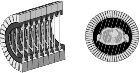
\includegraphics[width=0.5\textwidth]{figs/fig_pet_parallel.pdf}
\caption{\label{fig:pet_parallel} \emph{Raw PET data can be organized in
parallel projections, similar as in the gamma camera.}}
\end{figure}

\begin{figure}[tb]
\centering
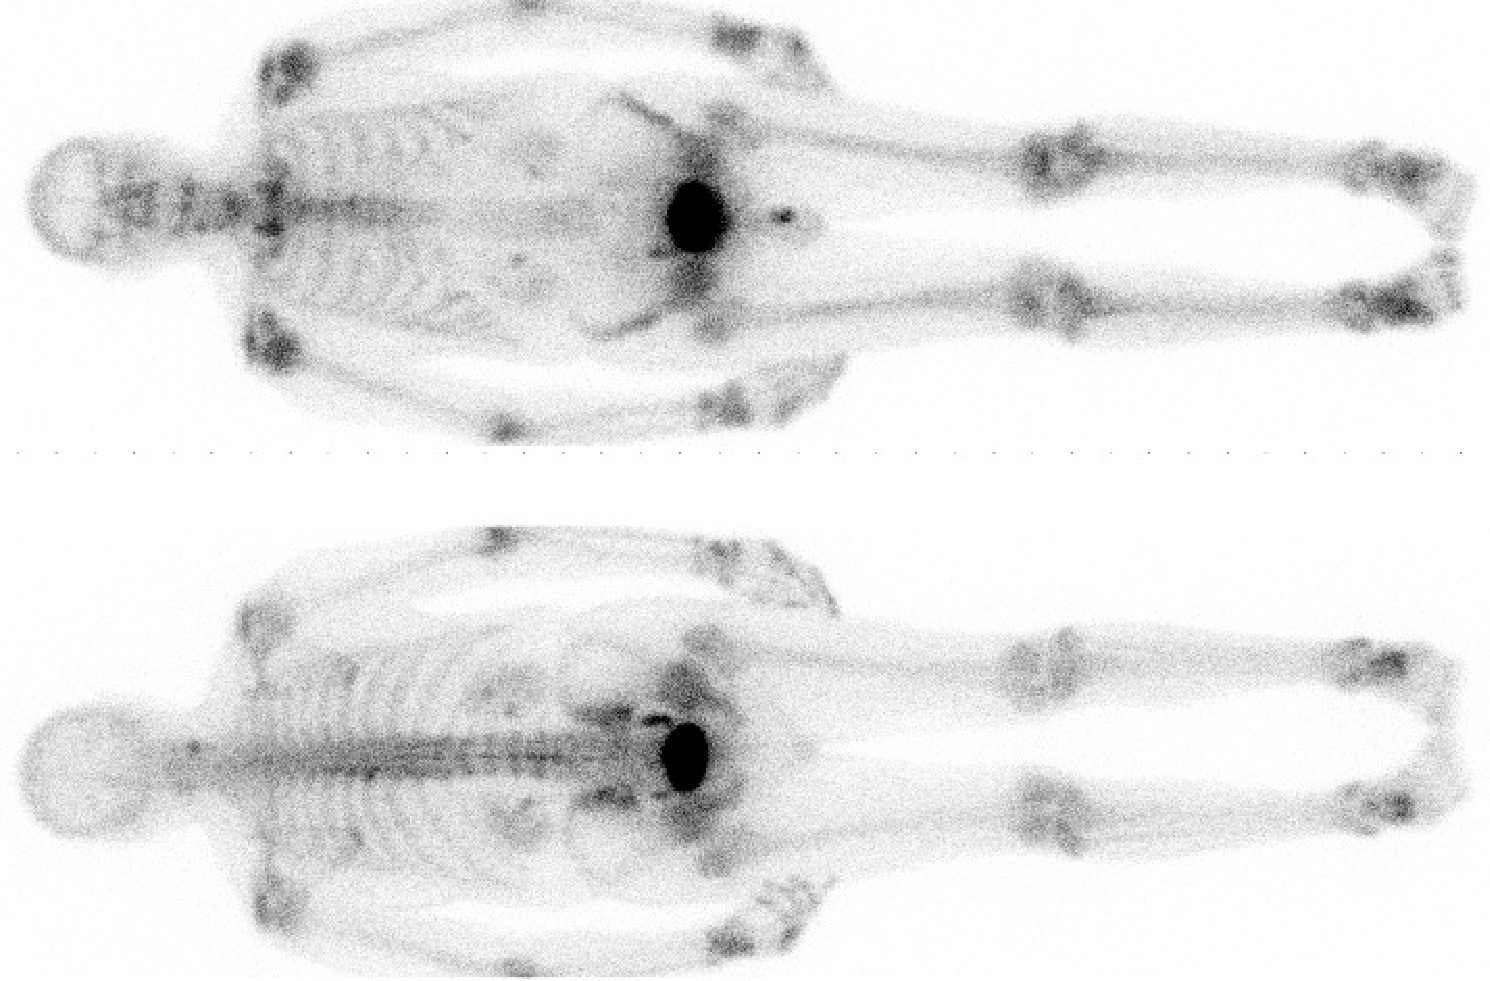
\includegraphics[width=0.5\textwidth]{figs/fig_jnwb.pdf}
\caption{\label{fig:planarwb} \emph{\textsuperscript{99m}Tc-MDP study acquired on a dual
head gamma camera. Detector size is about 40 $\times$ 50 cm, the whole body
images are acquired with slow translation of the patient bed. MDP accumulates
in bone, allowing visualization of increased bone metabolism. Due to
attenuation, the spine is better visualized on the posterior image.}}
\end{figure}

Figure \ref{fig:planarwb} shows a planar whole body image, which is obtained
by slowly moving the gamma camera over the patient and combining the
projections into a single image. In this case, a gamma camera with two opposed
detector heads was used, so the posterior and anterior views are acquired
simultaneously. There is no rotation, these are simply raw data, but they
provide valuable diagnostic information. A similar approach is applied in
radiological studies: with the CT tomographic images can be produced, but the
planar images (e.g. thorax X-ray) already provide useful information. 

\begin{figure}[tb]
\centering
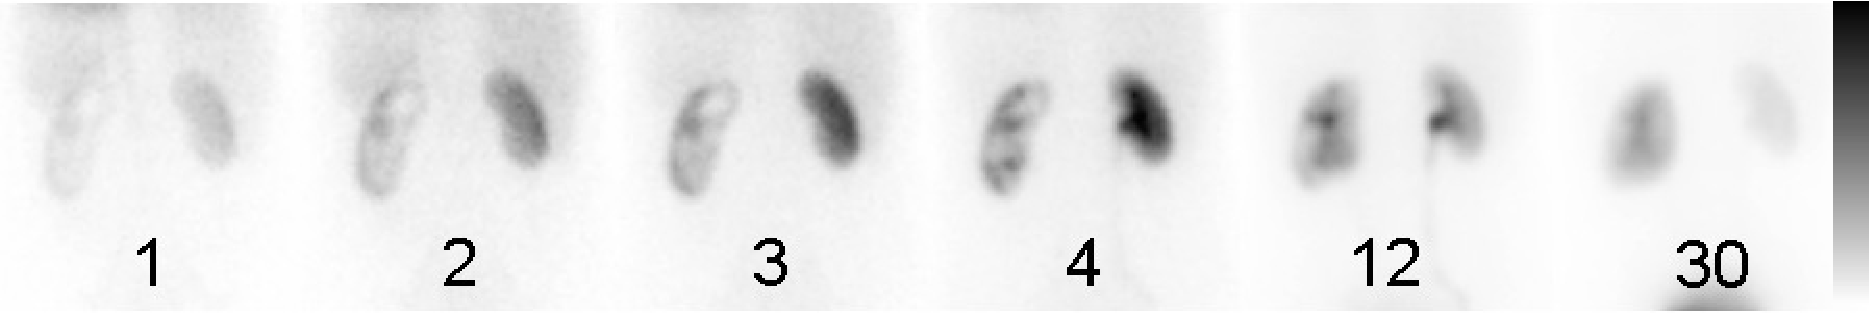
\includegraphics[width=0.9\textwidth]{figs/fig_renaldynimg.pdf}
\caption{\label{fig:renaldyn} \emph{A few images from a
    renography. The numbers are the minutes after injection of the
    \textsuperscript{99m}Tc-labeled tracer. The left kidney (at the right in the
    image) is functioning normally, the other one is not: both uptake
    and clearance of the tracer are slowed down.}}
\end{figure}

\begin{figure}[tb]
\centering
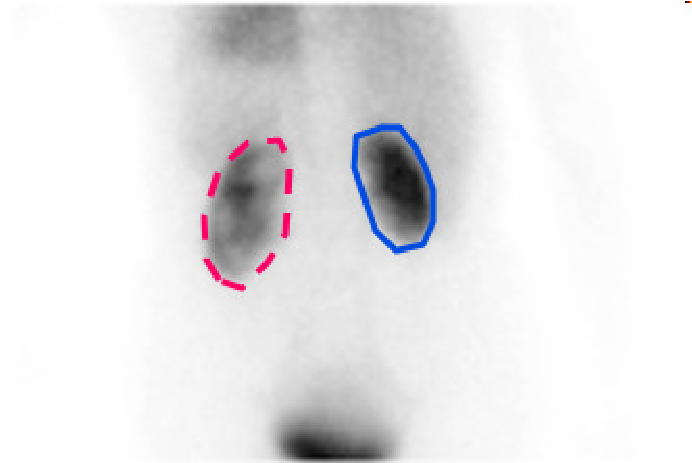
\includegraphics[width=0.45\textwidth]{figs/fig_renalrois.pdf}
  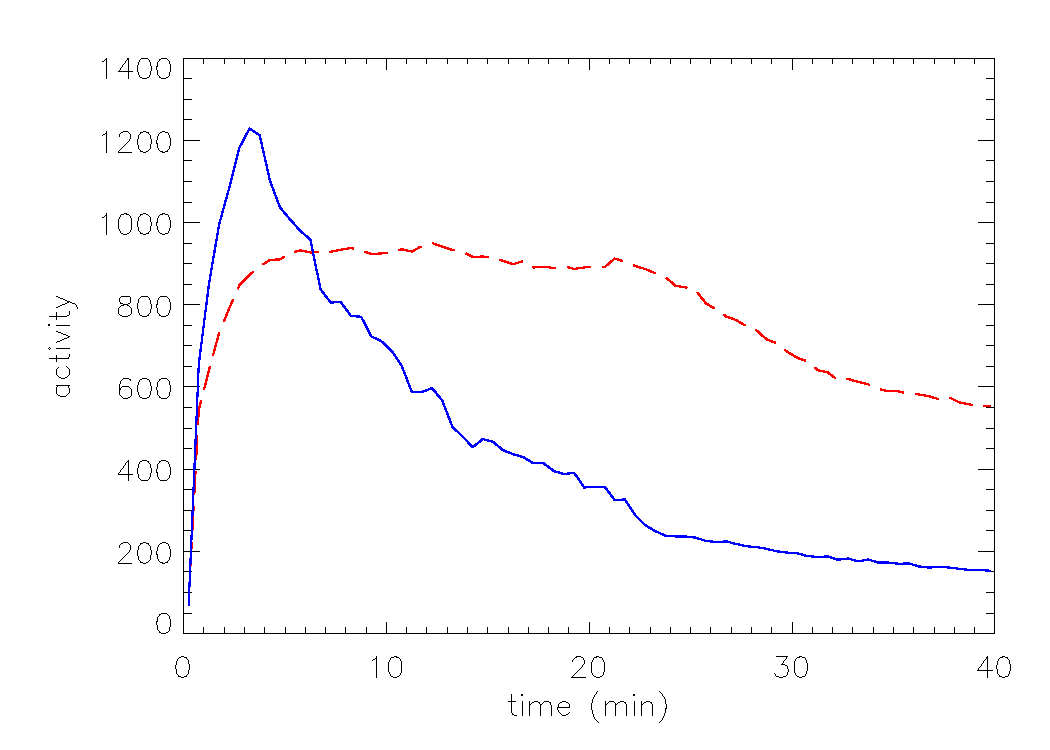
\includegraphics[width=0.5\textwidth]{figs/fig_renalplot.pdf}
\caption{\label{fig:renalroi} \emph{Summing all frames of the dynamic
    renal study yields the image on the left, where the kidneys can be
    easily delineated. The total count in these regions as a function
    of time (time activity curves or TACs) are shown on the right,
    revealing a distinct difference in kidney function.}}
\end{figure}

The dynamic behaviour of the tracer can be measured by acquiring a
series of consecutive images. To study the function of the kidneys, a
\textsuperscript{99m}Tc\ labeled tracer (in this example ethylene dicysteine, known
as \textsuperscript{99m}Tc-EC) is injected, and its renal uptake is studied over
time. The first two minutes after injection, 120 images of 1 s are
acquired to study the perfusion. Then, about a hundred planar images
are acquired over 40 min to study the clearance. Fig
\ref{fig:renaldyn} and \ref{fig:renalroi} show the results in a
patient with one healthy and one poorly functioning kidney.

The study duration should not be too long because of patient
comfort. A scanning time of 15 min or half an hour is reasonable, more
is only acceptable if unavoidable. If that time is used to acquire a
single or a few planar images, there will be many photons per pixel
resulting in good signal to noise ratio, but there is no depth
information.  If the same time is used to acquire many projections for
tomographic reconstruction, then there will be few counts per pixel
and more noise, but we can reconstruct a three-dimensional image of
the tracer concentration. The choice depends on the application.

In contrast, planar PET studies are very uncommon, because most PET-cameras
are acquiring all projections simultaneously, so the three-dimensional image
can always be reconstructed.

\section{2D Emission Tomography}
%%%%%%%%%%%%%%%%%%%%%%%
% Sinogram
% FBP
% MLEM
% Randoms correction
% Scatter correction
% Collimator blurring

In this section, we will study the reconstruction of a planar distribution
from its line integrals. The data are two-dimensional: a projection line is
completely specified by its angle and its distance to the center of the field
of view. A two-dimensional image that uses $d$ as the column coordinate and
$\theta$ as the row coordinate is called a {\em sinogram}. Figure
\ref{fig:sinogram} shows that the name is well chosen: the sinogram of point
source is zero everywhere except on a sinusoidal curve. The sinogram in the
figure is for 180\textdegree. A sinogram for 360\textdegree\ shows a full period of
the sinusoidal curve. It is easy to show that, using the conventions of figure
\ref{fig:sinogram}, $s(x,y) = s_x + s_y = x \cos \theta + y \sin \theta$, so
the non-zero projections in the sinogram are indeed following a sinusoidal
curve.

\begin{figure}[tb]
\centering
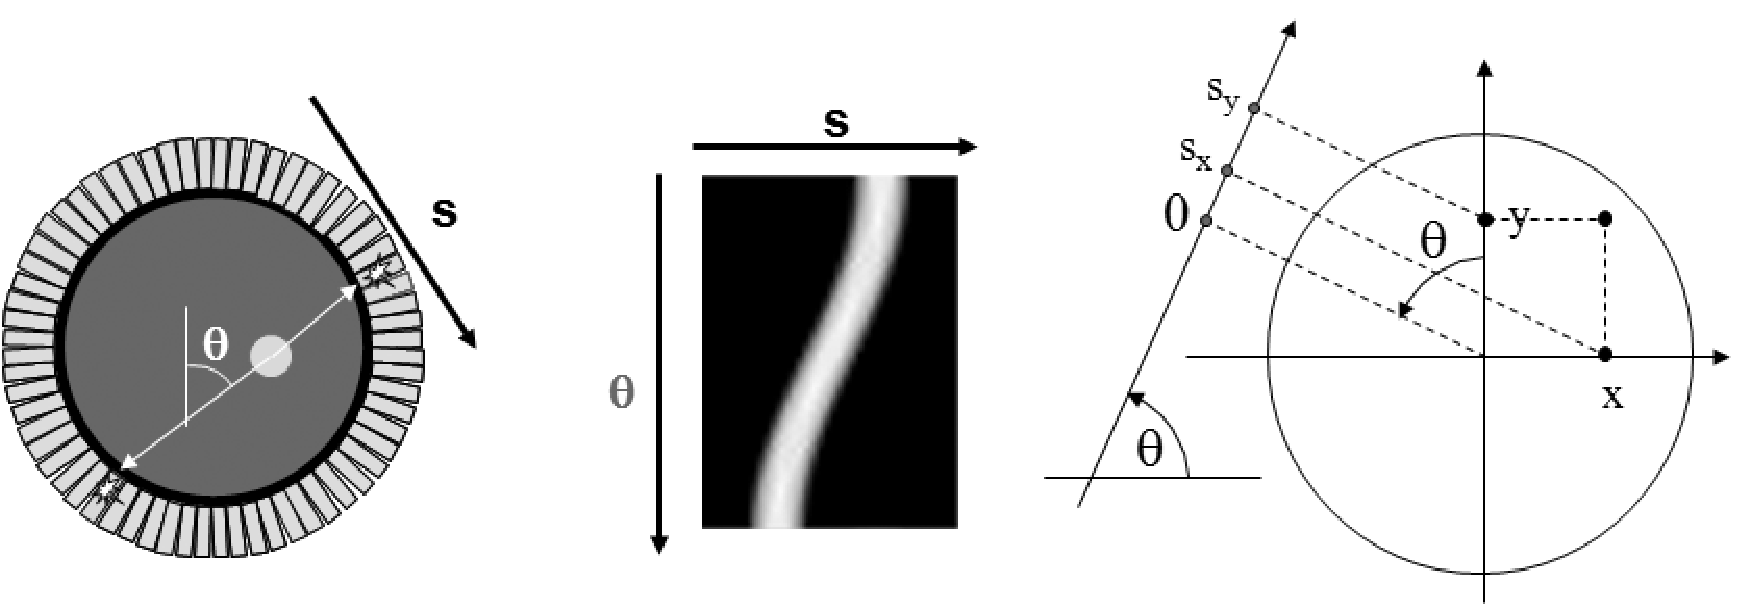
\includegraphics[width=0.9\textwidth]{figs/fig_sinogram.pdf}
\caption{\label{fig:sinogram} \emph{A sinogram is obtained by storing the 1D
parallel projections as the rows in a matrix (or image). Left: the camera with
a radioactive disk. Center: the corresponding sinogram. Right: the
conventions, $\theta$ is positive in clockwise direction.}}
\end{figure}

\subsection{2D filtered backprojection}
%=================================
Filtered backprojection (FBP) is the mathematical inverse of an idealized
acquisition model: it computes a two-dimensional continuous distribution from
ideal projections. In this case, ``ideal'' means the following:
\begin{itemize}
\item
The distribution has a finite support: it is zero, except within a finite
region.  We assume this region is circular (we can always do that, since the
distribution must not be non-zero within the support). We assume that this
region coincides with the field of view of the camera. We select the center of
the field of view as the origin of a two-dimensional coordinate system.

\item
Projections are continuous: the projection is known for every angle and for
every distance from the origin. Projections are ideal: they are unweighted
line integrals (so there is no attenuation and no scatter, the PSF is a Dirac
impulse and there is no noise).

\item
The distribution is finite everywhere. That should not be a problem in real
life.

\end{itemize}

\subsubsection{Projection}
%------------------------------------
\begin{figure}[tb]
\centering
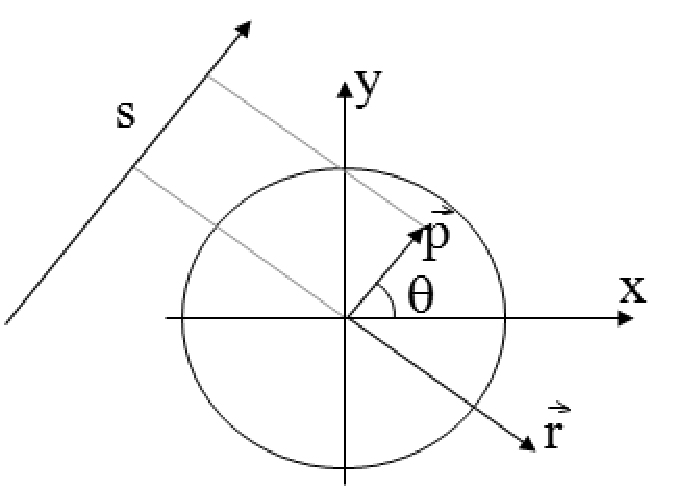
\includegraphics[width=0.35\textwidth]{figs/fig_fbp_math.pdf}
\caption{\label{fig:fbp_math} \emph{The projection line as a function of a
single parameter $r$. The line consists of the points $\vec{p} + \vec{r}$,
with $\vec{p} = (s \cos \theta, s \sin \theta)$, $\vec{r} = (r \sin \theta, - r
\cos \theta)$.}}
\end{figure}

Such an ideal projection $q$ is then defined as follows (using the conventions
of figure \ref{fig:sinogram}):
\begin{align}
q(s, \theta) &= \int_{(x,y) \in \; \mbox{projection line}}
                  \lambda(x,y) dx dy\\
             &= \int_{-\infty}^{\infty}
        \lambda(s \cos \theta + r \sin \theta,
                s \sin \theta - r \cos \theta) dr. \label{eq:jnidealproj}
\end{align}
The point $(s \cos \theta, s \sin \theta)$ is the point on the projection line
closest to the center of the field of view.  By adding $(r \sin \theta, - r
\cos \theta)$ we take a step $r$ along the projection line (fig
\ref{fig:fbp_math}).


\subsubsection{The Fourier theorem}
%------------------------------------
The Fourier theorem (also called the {\em central slice theorem})
states that there is a simple relation between the one-dimensional
Fourier transform of the projection $q(s, \theta)$ and the
two-dimensional Fourier transform of the distribution $\lambda(x,y)$.

The Fourier theorem is very easy to prove for projection along the y-axis (so
$\theta = 0$). Because the y-axis may be chosen arbitrarily, it holds for
any other projection angle (but the notation gets more elaborate).
In the following $Q$ is the 1-D Fourier transform (in the first coordinate) of
$q$. Because the angle is fixed and zero, we have
$q(s, \theta) = q(s, 0) = q(x,0)$.
\begin{align}
  q(x,0) &= \int_{-\infty}^{\infty} \lambda(x,y) dy \\
  Q(\nu_x,0) &= \int_{-\infty}^{\infty}  q(x,0) e^{-j2\pi \nu_x x} dx \\
          &= \int_{-\infty}^{\infty}  \int_{-\infty}^{\infty}
                 \lambda(x,y) e^{-j2\pi \nu_x x} dx dy.
\end{align}
Here, $j = \sqrt{-1}$. Let us now compute the 2-D Fourier transform
$\Lambda$ of $\lambda$:
\begin{equation}
\Lambda(\nu_x, \nu_y)  =   \int_{-\infty}^{\infty}  \int_{-\infty}^{\infty}
         \lambda(x,y) e^{-j2\pi (\nu_x x + \nu_y y)} dx dy.
\end{equation}
So it immediately follows that $\Lambda(\nu_x, 0) = Q(\nu_x)$.
Formulated for any angle $\theta$ this becomes:
\begin{equation}
  \Lambda(\nu \cos \theta, \nu \sin \theta) = Q(\nu, \theta). 
  \label{fouriertheorem}
\end{equation}
A more rigorous proof for any angle $\theta$ is given in appendix
\ref{app:cs}.  In words: the 1-D Fourier transform of the projection
acquired for angle $\theta$ is identical to a central profile along
the same angle through the 2-D Fourier transform of the original
distribution (fig \ref{fig:fouriertheorem}).

\begin{figure}[tb]
\centering
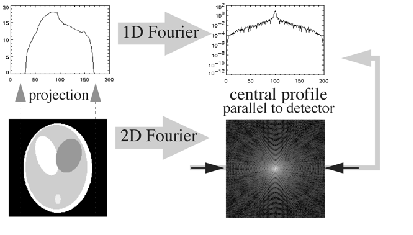
\includegraphics[width=0.6\textwidth]{figs/fig_fouriertheorem.pdf}
\caption{\emph{The Fourier theorem.}}
\label{fig:fouriertheorem} 
\end{figure}

The Fourier theorem directly leads to a reconstruction algorithm by simply
digitizing everything: compute the 1D FFT transform of the projections for
every angle, fill the 2D FFT image by interpolation between the radial 1D FFT
profiles, and compute the inverse 2D FFT to obtain the original distribution.

Obviously, this will only work if we have enough data. Every projection
produces a central line through the origin of the 2D frequency space. We need
to have an estimate of the entire frequency space, so we need central lines
over at least 180 degrees (more is fine but redundant).  Figure
\ref{fig:jnproj_sino} shows clinical raw emission data acquired for
tomography. They can be organized either as projections or as
sinograms. There are typically in the order of 100 (SPECT) or a few hundreds
(PET) of projection angles. The figure shows 9 of them. During a clinical
study, the gamma camera automatically rotates around the patient to acquire
projections over 180\textdegree or 360\textdegree. Because the spatial resolution
deteriorates rapidly with distance to the collimator, the gamma camera not
only rotates, it also moves radially as close as possible to the patient to
optimize the resolution.

As mentioned before, the PET camera consisting of detector rings measures all
projection lines simultaneously, no rotation is required.

\begin{figure}[tb]
\centering
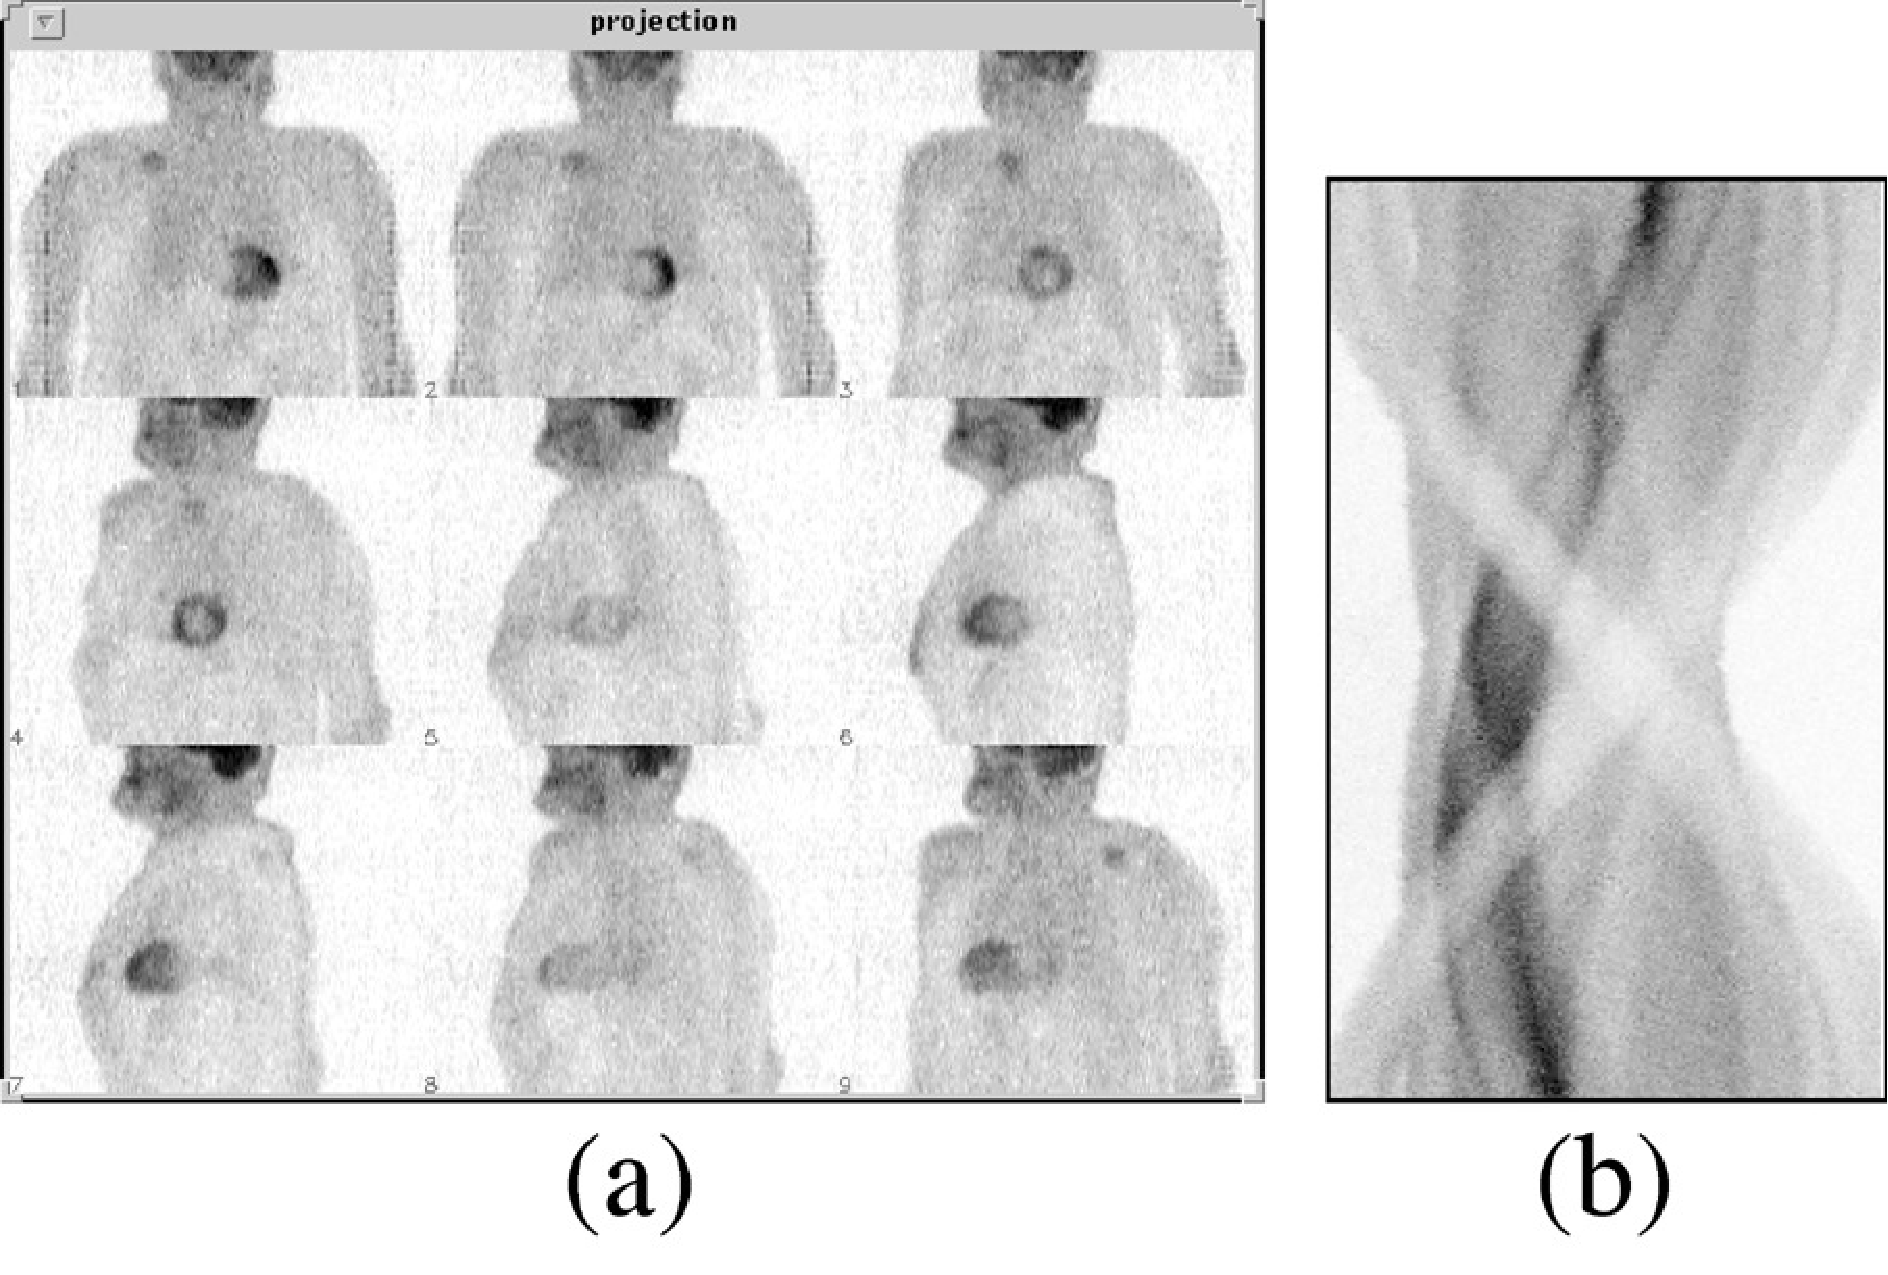
\includegraphics[width=0.72\textwidth]{figs/fig_jnproj_sino.pdf}
\caption{\label{fig:jnproj_sino} \emph{Raw PET data, organized as projections
(a) or as a sinogram (b). There are typically a few hundred projections, one
for each projection angle, and several tens to hundred sinograms, one
for each slice through the patient body}}
\end{figure}


\subsubsection{Backprojection} \label{sec:backprojection}
%------------------------------------
This Fourier-based reconstruction works, but usually an alternative expression
is used, called ``filtered backprojection''. To explain it, we must first define
the operation {\em backprojection}:
\begin{align}
 b(x,y) &= \int_0^\pi q(x \cos \theta + y \sin \theta, \theta) d \theta
             \nonumber\\
      &= \mbox{Backproj} \left( q(s, \theta) \right). \label{eq:jnbackproj}
\end{align}

\begin{figure}[tb]
\centering
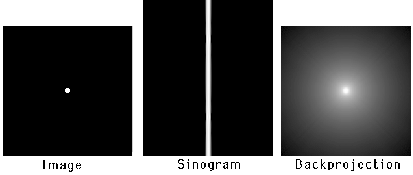
\includegraphics[width=0.6\textwidth]{figs/fig_backproj.pdf}
\caption{\label{fig:backproj} \emph{A point source, its sinogram and the
backprojection of the sinogram (logarithmic gray value scale).}}
\end{figure}

During backprojection, every projection value is uniformly distributed
along its projection line. Since there is exactly one projection line
passing through $(x,y)$ for every angle, the operation involves
integration over all angles. This operation is {\em NOT} the inverse
of the projection. As we will see later on, it is the {\em adjoint
operator} of projection. Figure \ref{fig:backproj} shows the
backprojection image using a logarithmic gray value scale. The
backprojection image has no zero pixel values!

Let us compute the values of the backprojection image from the
projections of a point source. Because the point is in the origin, the
backprojection must be radially symmetrical. The sinogram is zero
everywhere except for $s = 0$ (fig \ref{fig:backproj}), where it is
constant, say $A$. So in the backprojection we only have to consider the
central projection lines, the other lines contribute nothing to the
backprojection image.  Consider the line integral along a circle
around the center (that is, the sum of all values on the circle). The
circle intersects every central projection line twice, so the total
activity the circle receives during backprojection is
\begin{equation}
  \mbox{total circle value} = 2 \int_0^\pi q(0, \theta) d \theta = 2 A\pi.
  \label{eq:bprojvalue}
\end{equation}
So the line integral over a circle around the origin is a constant. The value
in every point of a circle with radius $R$ is $2 A \pi / (2 \pi R) =
A/R$. In conclusion, starting with an image $f(x,y)$ which is zero everywhere,
except in the center where it equals $A$, we find:
\begin{align}
  f(x,y) &= A \delta(x) \delta(y)\\
 b(x,y) &= (\mbox{backproj}(\mbox{proj}(f))(x,y) \; = \;
  \frac{A}{\sqrt{x^2 + y^2}}.
\end{align}
A more rigorous derivation is given in appendix \ref{app:bprojproj}.

Projection followed by backprojection is a linear operation. In the
idealized case considered here, it is also a shift invariant
operation. Consequently, we have actually computed the point spread function
of that operation.

\subsubsection{Filtered backprojection}
%------------------------------------
Filtered backprojection follows directly from the Fourier theorem:
\begin{align}
  \lambda(x,y) &= \int_{-\infty}^{\infty} \int_{-\infty}^{\infty}
         \Lambda(\nu_x, \nu_y) e^{j2\pi (\nu_x x + \nu_y y)} d \nu_x d \nu_y\\
      &\Downarrow \mbox{Polar transform:} d \nu_x d \nu_y = |\nu|
         d\nu d\theta \nonumber\\
      &= \int_{-\infty}^{\infty} d\nu \int_0^\pi |\nu| d\theta
            \Lambda(\nu \cos \theta, \nu \sin \theta)
            e^{j2\pi \nu (x \cos \theta + y \sin \theta)}\\
      &\Downarrow \mbox{Fourier theorem and switching integral signs}
               \nonumber\\
      &= \int_0^\pi d\theta \int_{-\infty}^{\infty} |\nu| d\nu
            Q(\nu, \theta) e^{j2\pi \nu (x \cos \theta + y \sin \theta)}\\
      &\Downarrow \mbox{Apply definition of backprojection} \nonumber\\
      &= \mbox{Backproj} \left( \int_{-\infty}^{\infty}
            |\nu| Q(\nu, \theta) e^{j2\pi \nu x} d\nu \right)\\
      &= \mbox{Backproj}\left( \mbox{Rampfilter} \left( q(s,\theta) \right)
            \right).
\end{align}
The ramp filter is defined as the sequence of 1D Fourier transform,
multiplication with the ``ramp'' $| \nu |$ and inverse 1D Fourier
transform.  To turn it into a computer program that can be applied to
a real measurement, everything is digitized and 1D Fourier is replaced
with 1D FFT. The ramp filter can also be implemented in the spatial
domain:
\begin{equation}
  \lambda(x,y) = \mbox{Backproj}\left( \mbox{inverse-Fourier-of-Rampfilter} 
                  \otimes q(s, \theta) \right),
\end{equation}
where $\otimes$ denotes convolution. This convolution filter is
obtained by taking the inverse Fourier transform of the ramp filter,
which is done in appendix \ref{app:ramp}. The ramp filter and the
corresponding convolution mask are shown in figure
\ref{fig:rampfilter}.

One can regard the ramp filter as a high pass filter which is designed to undo
the blurring caused by backprojecting the projection, where the blurring mask
is the point spread function computed in section \ref{sec:backprojection}.

Mathematically, filtered backprojection is identical to Fourier-based
reconstruction, so the same conditions hold: e.g. we need projections over 180
degrees. Note that after digitization, the algorithms are no longer identical.
The algorithms have different numerical properties and will produce slightly
different reconstructions. Similarly, implementing the ramp filter in the
Fourier domain or as a spatial convolution will produce slightly different
results after digitization. 
%
\begin{figure}[tb]
%\centering
  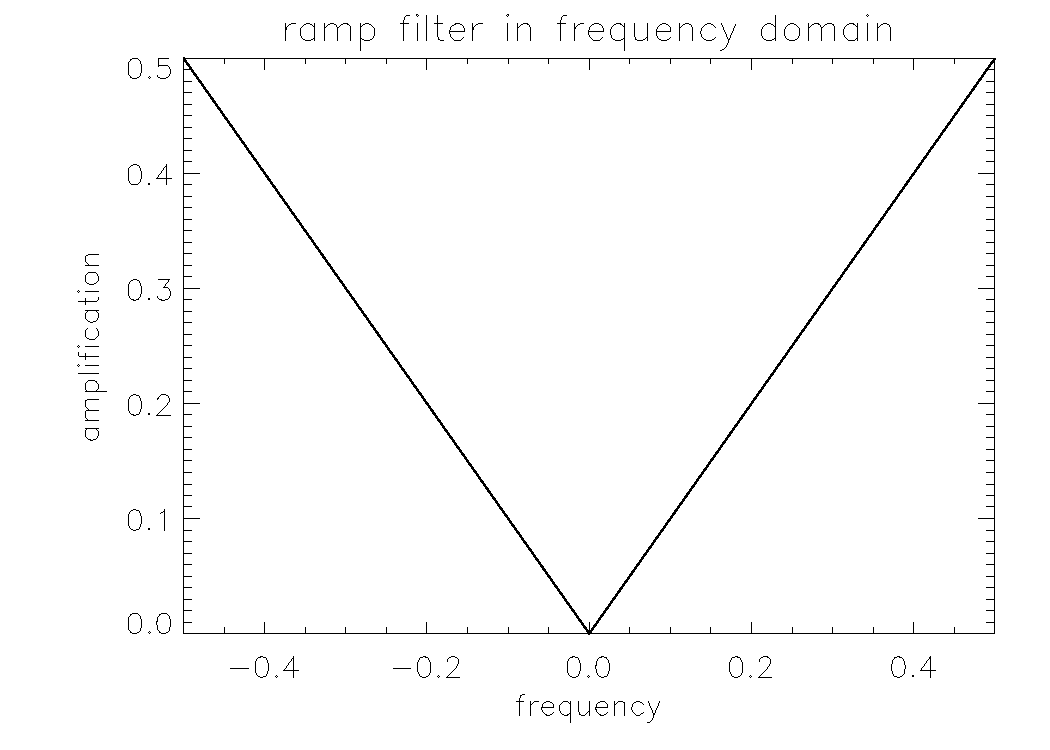
\includegraphics[width=0.45\textwidth]{figs/fig_rampfilter1.pdf}
  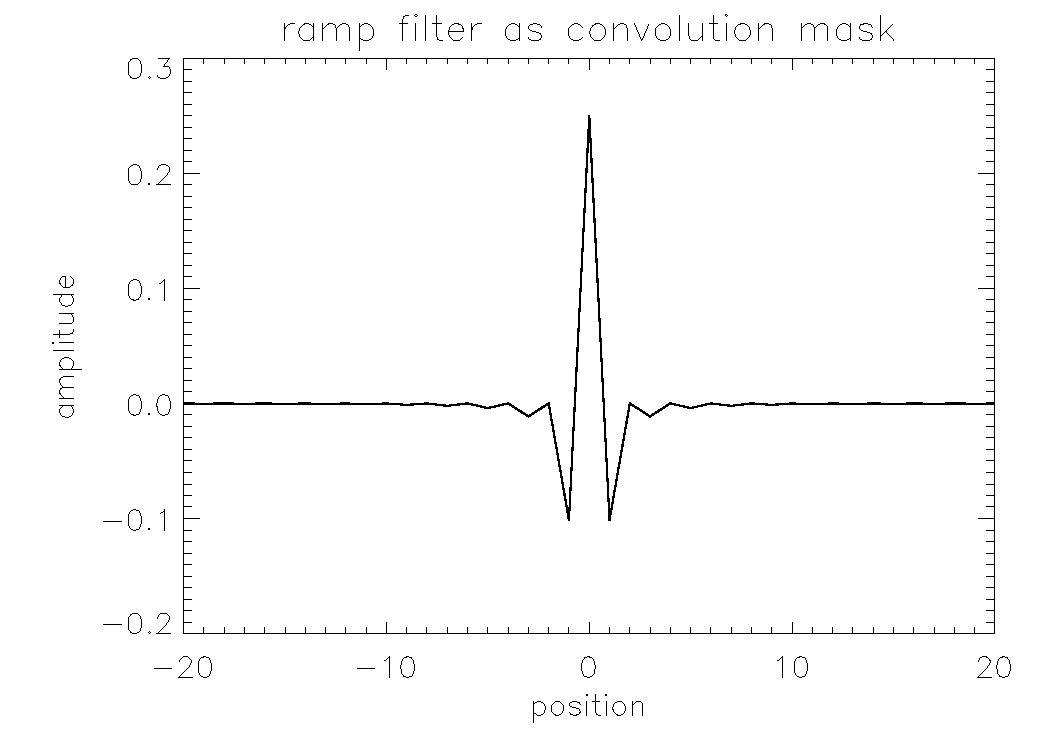
\includegraphics[width=0.45\textwidth]{figs/fig_rampfilter2.pdf}
\caption{\label{fig:rampfilter} \emph{The rampfilter in the frequency
    domain (left) and its point spread function (right). The latter is
    by definition also the mask needed to compute the filter with a
    convolution in the spatial domain.}}
\end{figure}

The ramp filter obviously amplifies high frequencies. If the
projection data are noisy, the reconstructed image will suffer from
high frequency noise. To reduce that noise, filtered backprojection is
always applied in combination with a smoothing (low pass) filter.

\subsubsection{Attenuation correction} \label{sec:attencor}
%------------------------------------
From a CT-measurement, we can directly compute a sinogram of line integrals.
Starting from eq (\ref{eq:ct_proj}) we obtain:
\begin{equation}
  \ln \frac{t_0}{t(b)} = \int_a^b \mu(s) ds. \label{eq:attencor}
\end{equation}
CT measurements have low noise and narrow PSF, so filtered backprojection
produces good results in this case. For emission tomography, the assumptions
are not valid. Probably the most important deviation from the FBP-model is the
presence of attenuation.

Attenuation cannot be ignored. E.g. at 140 keV, every 5 cm of tissue eliminates
about 50\% of the photons. So in order to apply filtered backprojection, we
should first correct for the effect of attenuation. In order to do so, we have
to know the effect. This knowledge can be obtained with a measurement.
Alternatively, we can in some cases obtain a reasonable estimate of that effect
from the emission data only.

In order to measure attenuation, we can use an external radioactive source
rotating around the patient, and use the SPECT or PET system as a CT-camera to
do a transmission measurement. If the external source emits $N_0$ photons
along the x-axis, the expected fraction of photons making it through the
patient is:
\begin{equation}
\frac{N(d)}{N_0} = e^{-\int_a^d \mu(x) dx} \label{eq:ct_proj2}.
\end{equation}
This is identical to the attenuation-factor in the PET-projection, equation
(\ref{eq:pet_proj}). So we can correct for attenuation by multiplying the
emission measurement $q(d)$ with the correction factor $N_0 / N(d)$.
For SPECT (equation (\ref{eq:spect_proj})), this is not possible.

In many cases, we can assume that attenuation is approximately constant (with
known attenuation coefficient $\mu$) within the body contour. Often, we can
obtain a fair body contour by segmenting a reconstruction obtained without
attenuation correction. In that case, (\ref{eq:ct_proj2}) can be computed from
the estimated attenuation image.

Bellini has adapted filtered backprojection for constant SPECT-like attenuation
within a known contour in 1979. The inversion of the general attenuated Radon
transform (i.e. reconstruction for SPECT with arbitrary (but known) attenuation) has
been studied extensively, but only in 2000 Novikov found a solution. The solution
came a bit late in fact, because by then, iterative reconstruction had replaced
analytical reconstruction as the standard approach in SPECT. And in iterative
reconstruction, non-uniform attenuation poses no particular problems.

\subsection{Iterative Reconstruction} \label{sec:iterrecon}
%====================================
Filtered backprojection is elegant and fast, but not very
flexible. The actual acquisition differs considerably from the ideal
projection model, and this deviation causes reconstruction
artifacts. It has been mentioned that attenuation correction in SPECT
may be problematic, but there are other deviations from the ideal line
integral: the measured projections are not continuous but discrete,
they contain a significant amount of noise (Poisson noise), the point
spread function is not a Dirac impulse and Compton scatter may
contribute significantly to the measurement.

That is why many researchers have been studying iterative algorithms. The nice
thing about these algorithms is that they are not based on mathematical
inversion.  All they need is a mathematical model of the acquisition, not its
inverse. Such a forward model is much easier to derive and program. That
forward model allows the algorithm to {\em evaluate} any reconstruction, and
to {\em improve} it based on that evaluation. If well designed, iterative
application of the same algorithm should lead to continuous improvement, until
the result is ``good enough''.

There are many iterative algorithms, but they are rather similar, so
explaining one should be sufficient. In the following, the maximum-likelihood
expectation-maximization (ML-EM) algorithm is discussed, because it is
currently by far the most popular one.

The algorithm is based on a Bayesian description of the problem. In
addition, it assumes that both the solution and the measurement are
discrete. This is correct in the sense that both the solution and the
measurement are stored in a digital way. However, the true tracer
distribution is continuous, so the underlying assumption is that this
distribution can be well described with a discrete representation.

\subsubsection{Bayesian approach} \label{sec:bayes}
%--------------------------------
Assume that somehow we have computed the reconstruction $\Lambda$ from the
measurement $Q$. The likelihood that both the measurement and the
reconstruction are the true ones ($p(Q \; \mbox{and} \; \Lambda)$) can be
rewritten as:
\begin{equation}
  p(\Lambda | Q) p(Q) = p(Q | \Lambda) p(\Lambda).
\end{equation}
It follows that
\begin{equation}
   p(\Lambda | Q) = \frac{p(Q | \Lambda) p(\Lambda)}{p(Q)}. \label{eq:jnpost}
\end{equation}
This expression is known as {\em Bayes' rule}. The function
$p(\Lambda)$ is called {\em the prior}. It is the likelihood of an
image, without taking into account the data. It is only based on
knowledge we already have prior to the measurement. E.g. the
likelihood of a patient image, clearly showing that the patient has no
lungs and four livers is zero. The function $p(Q | \Lambda)$ is simply
called {\em the likelihood} and gives the probability to obtain
measurement $Q$ assuming that the true distribution is $\Lambda$. The
function $p(\Lambda | Q)$ is called {\em the posterior}. The
probability $p(Q)$ is a constant value, since the data $Q$ have been
measured and are fixed during the reconstruction.

Maximizing $p(\Lambda | Q)$ is called the {\em maximum-a-posteriori (MAP)}
approach. It produces ``the most probable'' solution. Note that this doesn't
have to be the true solution. We can only hope that this solution shares
sufficient features with the true solution to be useful for our purposes.

Since it is not trivial to find good mathematical expressions for the prior
probability $p(\Lambda)$, it is often assumed to be constant, i.e.\ it is
assumed that a priori all possible solutions have the same probability to be
correct.  Maximizing $p(\Lambda | Q)$ then reduces to maximizing the
likelihood $p(Q | \Lambda)$, which is easier to calculate.  This is called the
{\em maximum-likelihood (ML)} approach, discussed in the following.

\subsubsection{The likelihood function for emission tomography}
%--------------------------------------------------------------
We have to compute the likelihood $p(Q | \Lambda)$, assuming that the
reconstruction image $\Lambda$ is available and represents the true
distribution. In other words, how likely is it to measure $Q$ with a PET or
SPECT camera, when the true tracer distribution is $\Lambda$?

We start by computing what we would expect to measure. We have already
done that, it is the attenuated projection from equations
(\ref{eq:spect_proj}) and (\ref{eq:pet_proj}). However, we want a
discrete version here:
\begin{equation}
  r_i = \sum_{j=1,J} c_{ij} \lambda_j, \;\; i = 1,I.  \label{jn:mlproj}
\end{equation}
Here, $\lambda_j \in \Lambda$ is the regional activity present in the
volume represented by pixel $j$ (since we have a finite number of
pixels, we can identify them with a single index). The value $r_i$ is
the number of photons measured in detector position $i$ ($i$ combines
the digitized coordinates $(d,\theta,z)$, it identifies a single
projection line). The value $c_{ij}$ represents the sensitivity of
detector $i$ for activity in $j$. If we have good collimation,
$c_{ij}$ is zero everywhere, except for the $j$ that are intersected
by projection line $i$, so the matrix $C$, often called the system
matrix, is very sparse. This notation is very general, and allows us
e.g. to take into account the finite acceptance angle of the
mechanical collimator (which will increase the fraction of non-zero
$c_{ij}$). If we know the attenuation coefficients, we can include
them in the $c_{ij}$, and so on. Consequently, this approach is valid
for SPECT and PET.

We now have for every detector two values: the expected value $r_i$ and the
measured value $q_i$. Since we assume that the data are samples from a Poisson
distribution, we can compute the likelihood of measuring $q_i$, if $r_i$
photons were expected (see eq. (\ref{jn:Poisson})):
\begin{equation}
  p(q_i | r_i) = \frac{e^{-r_i} r_i^{q_i}}{q_i!}.
\end{equation}
The history of one photon (emission, trajectory, possible interaction with
electrons, possible detection) is independent of that of the other photons, so
the overall probability is the product of the individual ones:
\begin{equation}
  p(Q | \Lambda) = \prod_i \frac{e^{-r_i} r_i^{q_i}}{q_i!}. \label{jn:mllik}
\end{equation}

Obviously, this is going to be a very small number: e.g. $p(q_i = 15 | r_i =
15) = 0.1$ and smaller for any other $r_i$. For larger $q_i$, the maximum
$p$-value is even smaller. In a measurement for a single slice, we have in the
order of 10000 detector positions, so the maximum likelihood value may be in
the order of $10^{-10000}$, which is zero in practice. We are {\em sure} the
solution will be wrong. However, we hope it will be close enough to the true
solution to be useful.

Maximizing (\ref{jn:mllik}) is equivalent to maximizing its logarithm, since
the logarithm is monotonically increasing. When maximizing over $\Lambda$,
factors not depending on $\lambda_j$ can be ignored, so we will drop $q_i!$
from the equations. The resulting log-likelihood function is
\begin{align}
  L(Q | \Lambda) &= \sum_i q_i \ln(r_i) - r_i \\
        &= \sum_i q_i \ln(\sum_j c_{ij} \lambda_j) - \sum_j c_{ij}
           \lambda_j. \label{eq:likelihood}
\end{align}

It turns out that the Hessian (the matrix of second derivatives) is negative
definite if the matrix $c_{ij}$ has maximum rank. In practice, this means that
the likelihood function has a single maximum, provided that a sufficient amount
of different detector positions $i$ were used.

\subsubsection{Maximum-Likelihood Expectation-Maximization}
%----------------------------------------------------------
Since we can compute the first derivative (the gradient), many algorithms can
be devised to maximize $L$. A straightforward one is to set the first
derivative to zero and solve for $\lambda$.
\begin{equation}
 \frac{\partial L}{\partial \lambda_j} = \sum_i c_{ij} \left(
      \frac{q_i}{\sum_k c_{ik} \lambda_k} - 1 \right) = 0, \forall i = 1,I.
       \label{eq:jnmlgrad}
\end{equation}
This produces a huge set of equations, and analytical solution is not
feasible.

Iterative optimization, such as a gradient ascent algorithm, is a suitable
alternative.  Starting with an arbitrary image $\Lambda$, the gradient for
every $\lambda_j$ is computed, and a value proportional to that gradient is
added.  Gradient ascent is robust but can be very slow, so more sophisticated
algorithms have been investigated.

A very nice and simple algorithm with guaranteed convergence is the {\em
expectation- maximization (EM)} algorithm.  Although the resulting algorithm
is simple, the underlying theory is not. In the following we simply state that
convergence is proved and only show what the EM algorithm does. The interested
reader is referred to appendix \ref{app:em} for some notes on convergence.

\paragraph{Expected value of Poisson variables, given a single measurement
 \label{sec:expect_a_b}\\}
%''''''''''''''''''''''''''''''''''''''''''''''''''
The iterative algorithm described below makes use of the expected value of a
Poisson variable that contributes to a measurement. This section shows how
that value is computed. Consider the experiment of
fig \ref{fig:expected_a_b}: two vials containing a known amount of
radioactivity are put in front of a detector.
%
\begin{figure}[tb]
\centering
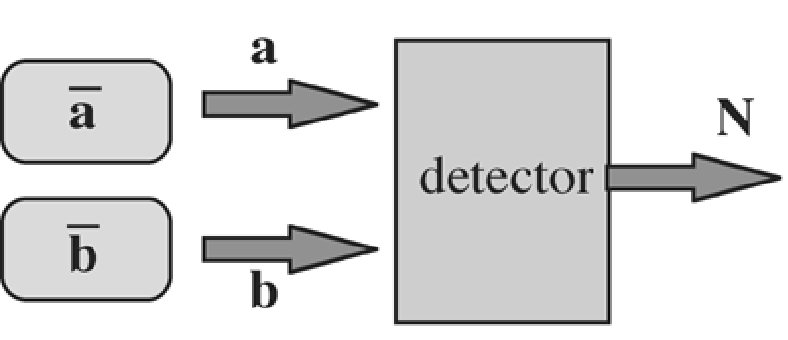
\includegraphics[width=0.4\textwidth]{figs/fig_expected_a_b.pdf}
\caption{\label{fig:expected_a_b} \emph{A detector measures the counts emitted
by two sources.}}
\end{figure}
%
Assume that we know the efficiency of the detector and its sensitivity for the
two vials, so that we can compute the expected amount of photons that each of
the vials will contribute during a measurement. The expected count is
$\bar{a}$ for vial 1 and $\bar{b}$ for vial 2. Now a single experiment is
carried out, and $N$ counts are measured by the detector.  Question: how many
photons $a$ and $b$ were emitted by each of the vials?

A-priori, we would expect $\bar{a}$ photons from vial 1 and $\bar{b}$ photons
from vial 2. But then the detector should have measured $\bar{a} + \bar{b}$
photons. In general, $N \neq \bar{a} + \bar{b}$ because of Poisson noise. So
the measurement $N$ supplies additional information, which we must use to
improve our expectations about $a$ and $b$. The answer is computed in appendix
\ref{app:expected_a_b}. The expected value of $a$, given $N$ is:
\begin{equation}
  E(a | a + b = N) = \bar{a} \frac{N}{\bar{a} + \bar{b}}, \label{eq:expect_a_b}
\end{equation}
and similar for $b$. So if more counts $N$ were measured than the expected
$\bar{a}+\bar{b}$, the expected value of the contributing sources is
``corrected'' with the same factor. Extension to more than two sources is
straightforward.

\paragraph{The complete variables\\}
%''''''''''''''''''''''''''''''''''
To maximize the likelihood (\ref{eq:likelihood}), a trick is applied
which at first seems to make the problem more complicated. We
introduce a so-called set of ``complete'' variables $X = \{ x_{ij}\}$,
where $x_{ij}$ is the (unknown) number of photons that have been
emitted in $j$ and detected in $i$. The $x_{ij}$ are not observable,
but if we would have known them, the observed variables $q_i$ could be
computed, since $q_i = \sum_j x_{ij}$. Obviously, the expected value
of $x_{ij}$, given $\Lambda$ is
\begin{equation}
  E(x_{ij} | \Lambda) =  c_{ij} \lambda_j
\end{equation}
We can now derive a log-likelihood function for the complete variables $X$, in
exactly the same way as we did for $L$ (the $x_{ij}$ obey Poisson
statistics, just as $q_i$). This results in:
\begin{equation}
  L_x(X, \Lambda) = \sum_i \sum_j ( x_{ij} \ln (c_{ij} \lambda_j) - 
                    c_{ij} \lambda_j) \label{eq:jnlx}
\end{equation}
The EM algorithm prescribes a two stage procedure (and guarantees that
applying it repeatedly leads to the maximisation of both $L_x$ and
$L$). It is an iterative algorithm, which starts from a given
image, called $\Lambda^{old}$, and computes an improved image
$\Lambda^{new}$. The two stages are:
\begin{enumerate}
\item Compute the function $E(L_x(X, \Lambda) | Q,
      \Lambda^{old})$. Given $\Lambda^{old}$ and $Q$, it is impossible
      to compute $L_x(X, \Lambda)$, since we don't know the values of
      $x_{ij}$. However, we can calculate its {\em expected} value,
      using the current estimate $\Lambda^{old}$. This is called the
      {\em E-step}.
\item Calculate a new estimate of $\Lambda$ that maximizes the function
      derived in the first step. This is the {\em M-step}.
\end{enumerate}

\paragraph{The E-step\\}
%'''''''''''''''''''''''
The E-step yields the following expressions:
\begin{align}
E(L_x(X, \Lambda) | Q, \Lambda^{old}) &= 
   \sum_i \sum_j ( n_{ij} \ln (c_{ij} \lambda_j) -  c_{ij} \lambda_j)
   \label{eq:jnestep1}\\
n_{ij} &= c_{ij} \lambda_j^{old} \frac{q_i}{\sum_k c_{ik} \lambda_k^{old}}
   \label{eq:jnestep2}
\end{align}
Equation (\ref{eq:jnestep1}) is identical to equation (\ref{eq:jnlx}), except
that the unknown $x_{ij}$ values have been replaced by their expected values
$n_{ij}$. We would expect that $n_{ij}$ equals $c_{ij}
\lambda_j^{old}$. However, we also know that the sum of all $c_{ij}
\lambda_j^{old}$ equals the number of measured photons $q_i$. This situation
is identical to the problem studied in section \ref{sec:expect_a_b}, and 
equation (\ref{eq:jnestep2}) is the straightforward extension of equation
(\ref{eq:expect_a_b}) for multiple sources.

\paragraph{The M-step\\}
In the M-step, we maximize this expression with respect to $\lambda_j$, by
setting the partial derivative to zero:
\begin{equation}
\frac{\partial}{\partial \lambda_j} E(L_x(X, \Lambda) | Q, \Lambda^{old})
   =  \sum_i \left( \frac{n_{ij}}{\lambda_j} - c_{ij} \right) = 0
\end{equation}
So we find:
\begin{equation}
 \lambda_j  =  \frac{\sum_i n_{ij}}{\sum_i c_{ij}} \label{eq:jnmstep}
\end{equation}
Substitution of equation (\ref{eq:jnestep2}) produces the ML-EM
algorithm:
\begin{equation}
  \lambda_j^{new}  =  \frac{\lambda_j^{old}}{\sum_i c_{ij}}
           \sum_i c_{ij}  \frac{q_i}{\sum_k c_{ik} \lambda_k^{old}}
           \label{eq:jnmlem}
\end{equation}

\paragraph{Discussion\\}

This equation has a simple intuitive explanation:
\begin{enumerate}
\item
The ratio $q_i / \sum_j c_{ij} \lambda_j^{old}$ compares the measurement to
its expected value, based on the current reconstruction. If the ratio is
1, the reconstruction must be correct. Otherwise, it has to be improved.

\item
The ratio-sinogram is backprojected. The digital version of the backprojection
operation is
\begin{equation}
  \mbox{backprojection of $f$ equals: } b_j = \sum_i c_{ij} f_i.
\end{equation}
We have seen the continuous version of the backprojection in
(\ref{eq:jnbackproj}). The digital version clearly shows that
backprojection is the transpose (or the adjoint) of projection
\footnote{The adjoint of a matrix is its conjugate transpose. Because
  the projection coefficients are real values, the adjoint of the
  projection matrix is its transpose.}
: the operations are identical, except that backprojection sums over $i$,
while projection sums over $j$. Note that if the projection takes
attenuation into account, the backprojection does so to. The
backprojection does not attempt to correct for attenuation (it is not
the inverse), it simply applies the same attenuation factors as in the
forward projection.

\item
Finally, the backprojected image is normalized and multiplied with the current
reconstruction image.  It is clear that if the measured and computed sinograms
are identical, the entire operation has no effect. If the measured projection
values are higher than the computed ones, the reconstruction values tend to
get increased.
\end{enumerate}

If the initial image is non-negative, then the final image will be
non-negative too, since all factors are non-negative. This is in most
applications a desirable feature, since the amount of radioactivity
cannot be negative.

Comparing with (\ref{eq:jnmlgrad}) shows that the ML-algorithm is really a
gradient ascent method. It can be rewritten as
\begin{equation}
 \lambda_j^{\mbox{new}} = \lambda_j 
    + \frac{\lambda_j}{\sum_i c_{ij}} \frac{\partial L}{\partial \lambda_j}.
\end{equation}
So the gradient is weighted by the current reconstruction value, which is
guaranteed to be positive (negative radioactivity is meaningless). To make it
work, we can start with any non-zero positive initial image, and iterate until
the result is ``good enough''. Fig. \ref{fig:jnfbpml} shows the filtered
backprojection and ML-EM reconstructions from the same dataset. (The image
shown is not the true maximum likelihood image, since iterations were stopped
early as discussed below).
\begin{figure}[tb]
\centering
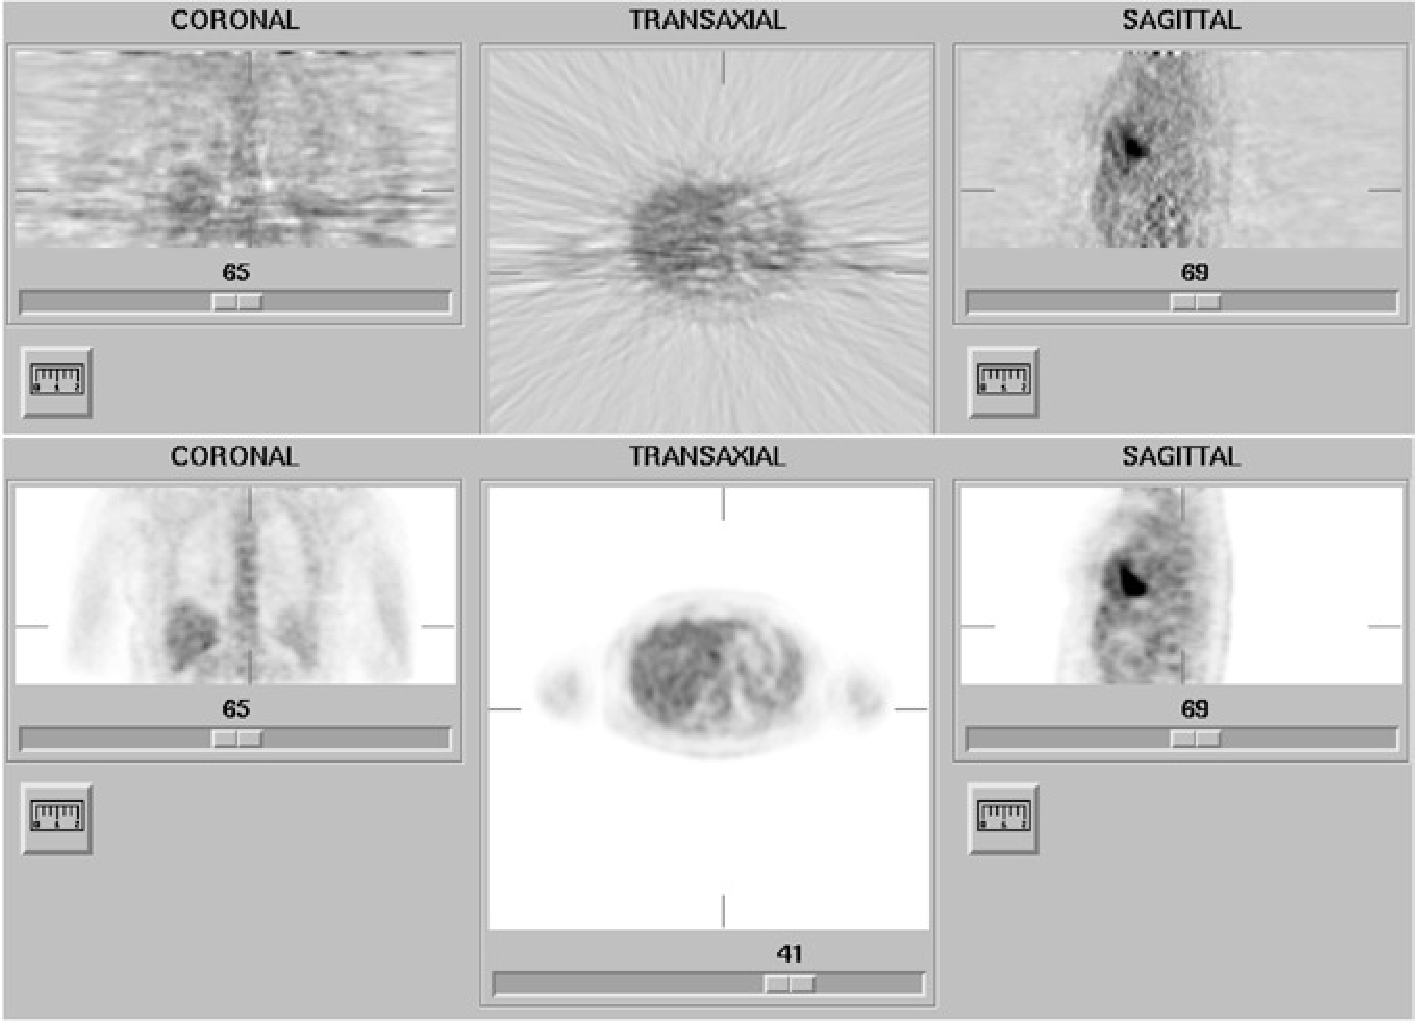
\includegraphics[width=0.72\textwidth]{figs/fig_jnfbpml.pdf}
\caption{\label{fig:jnfbpml} \emph{Reconstruction obtained with filtered
backprojection (top) and maximum-likelihood expectation-maximization (34
iterations) (bottom). The streak artifacts in the filtered backprojection
image are due to the statistical noise on the measured projection (Poisson
noise).}}
\end{figure}

\subsection{Compton scatter, random coincidences}
%================================================
As explained in section \ref{sec:randoms}, an estimate of the randoms
contribution to the PET sinogram can be obtained, e.g. with the
delayed window technique. Similarly, various methods exist to estimate
the scatter contribution in SPECT (section \ref{sec:spectscatcor})
and PET (section \ref{sec:petscatcor}). If an estimate of such an
additive contribution to the sinogram is available, it can be
incorporated in the ML-EM algorithm. The forward acquisition model
of (\ref{jn:mlproj}) is then extended as 
\begin{equation}
  r_i = \sum_{j=1,J} c_{ij} \lambda_j + s_i, \;\; i = 1 \ldots I,
  \label{jn:mlprojscat}
\end{equation}
where $s_i$ represents the estimate of the additive contribution from
scatter and/or randoms for projection line $i$. It can be shown that
the ML-EM algorithm then becomes
\begin{equation}
  \lambda_j^{new}  =  \frac{\lambda_j^{old}}{\sum_i c_{ij}}
           \sum_i c_{ij}  \frac{q_i}{\sum_k c_{ik} \lambda_k^{old} + s_i}
           \label{eq:jnmlemscat}
\end{equation}



\subsection{Regularization} \label{sec:regularization}
%==========================
Since the levels of radioactivity must be low, the number of detected photons
is also low. As a result, the uncertainty due to Poisson noise is important:
the data are often very noisy. 

Note that Poisson noise is ``white''. This means that its (spatial) frequency
spectrum is flat. Often this is hard to believe: one would guess it to be high
frequency noise, because we see small points, no blobs or a shift in mean
value.  That is because our eyes are very good at picking up high frequencies:
the blobs and the shift are there all right, we just don't see them.

Filtered backprojection has not been designed to deal with Poisson
noise. The noise propagates into the reconstruction, and in that
process it is affected by the ramp filter, so the noise in the
reconstruction is not white, it is truly high frequency noise. As a
result, it is definitely {\em not} Poisson noise. Figure
\ref{fig:jnfbpml} clearly shows that Poisson noise leads to streak
artifacts when filtered backprojection is used.

ML-EM does ``know'' about Poisson noise, but that does not allow it to separate
the noise from the signal. In fact, MLEM attempts to compute how many of the
detected photons have been emitted in each of the reconstruction pixels
$j$. That must produce a noisy image, because photon emission is a Poisson
process. What we really would like to know is the tracer concentration, which
is not noisy.

Because our brains are not very good at suppressing noise, we need to
do it with the computer. Many techniques exist. One can apply simple
smoothing, preferably in three dimensions, such that resolution is
approximately isotropic. It can be shown that for every isotropic 3D
smoothing filter applied after filtered backprojection, there is a 2D
smoothing filter, to be applied to the measured data before filtered
backprojection, which has the same effect. Since 2D filtering is
faster than 3D filtering, it is common practice to smooth before
filtered backprojection.

The same is not true for ML-EM: one should not smooth the measured projections,
since that would destroy the Poisson nature. Instead, the images are often
smoothed afterwards. Another approach is to stop the iterations before
convergence. ML-EM has the remarkable feature that low frequencies converge
faster than high ones, so stopping early has an effect similar to low-pass
filtering.

Finally, one can go back to the basics, and in particular to the
Bayesian expression (\ref{eq:jnpost}). Instead of ignoring the prior,
one can try and define some prior probability function that encourages
smooth solutions. This leads to maximum-a-posteriori (MAP)
algorithm. The algorithms can be very powerful, but they also have
many parameters and tuning them is a delicate task.

Although regularized (smoothed) images look much nicer than the original ones,
they do not contain more information. In fact, they contain less information,
since low-pass filtering kills high-frequency information and adds nothing
instead! Deleting high spatial frequencies results in poorer resolution (wider
point spread function), so excessive smoothing is ill advised if you hope to
see small structures in the image.

\subsection{Convergence} \label{sec:mlemconverge}
%==========================
\begin{figure}[tb]
\centering
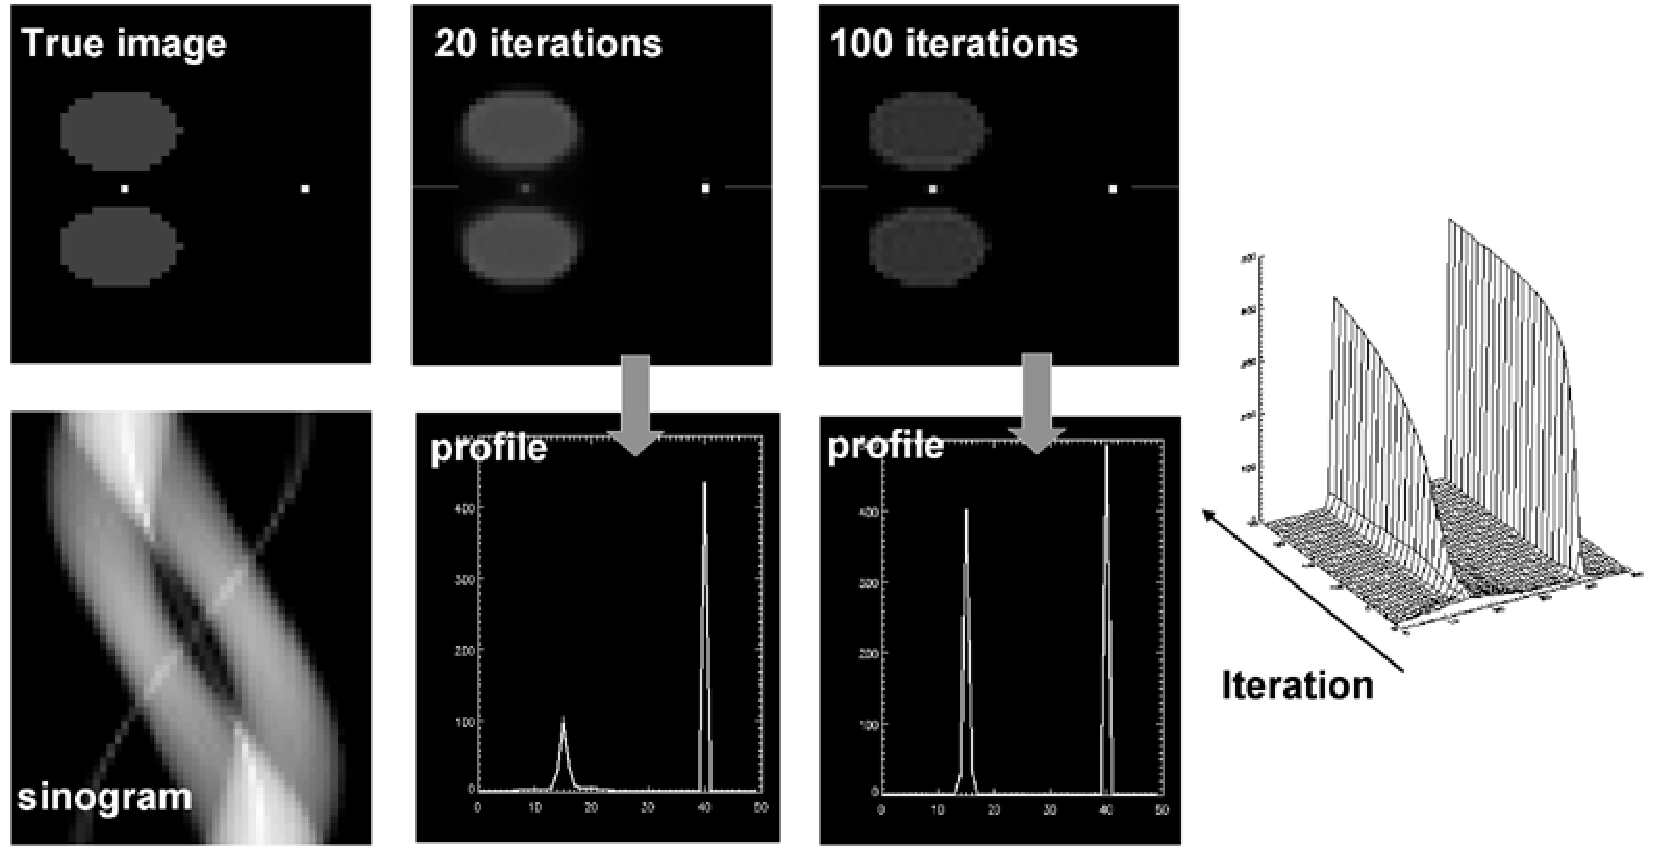
\includegraphics[width=0.9\textwidth]{figs/fig_mlem_converge.pdf}
\caption{\label{fig:mlem_converge} \emph{Simulation designed to challenge
convergence of MLEM: the point between the hot regions convergence very slowly
relative to the other point. The maximum converges slower than the width, so
counts are not preserved.}}
\end{figure}
%
Filtered backprojection is a linear algorithm with shift invariant point
spread function. That means that the effect of projection followed by filtered
backprojection can be described with a single PSF, and that the reconstruction
has a predictable effect on image resolution. Similarly, smoothing is linear
and shift invariant, so the combined effect of filtered backprojection with
low pass filtering has a known effect on the resolution.

In contrast to FBP, MLEM algorithm is non-linear and not shift invariant.
Stated otherwise, if an object is added to the reconstruction, then the effect
of projection followed by reconstruction is different for {\em all} objects in
the image. In addition, two identical objects can be reconstructed differently
because they are at a different position. In this situation, it is impossible
to define a PSF, projection followed by MLEM-reconstruction cannot be modeled
as a convolution. There is no easy way to predict the effect of MLEM on image
resolution. 

It is possible to predict the resolution of the true maximum likelihood
solution, but you need an infinite number of iterations to get
there. Consequently, if iterations are stopped early, convergence may be
incomplete. There is no way to tell that from the image, unless you knew
a-priori what the image was: MLEM images always look nice. So stopping
iterations early in patient studies has unpredictable consequences.

This is illustrated in a simulation experiment shown in figure
\ref{fig:mlem_converge}. There are two point sources, one point source is
surrounded by large active objects, the other one is in a cold region. After
20 MLEM iterations, the ``free'' point source has nearly reached its final
value, while the other one is just beginning to appear. Even after 100
iterations there is still a significant difference. The difference in
convergence affects not only the maximum count, but also the total count in a
region around the point source.

Consequently, it is important to apply ``enough'' iterations, to get
``sufficiently'' close to the true ML solution. In the previous section it was
mentioned that stopping iterations early has a noise-suppressing effect. 
%
\begin{figure}[tb]
\centering
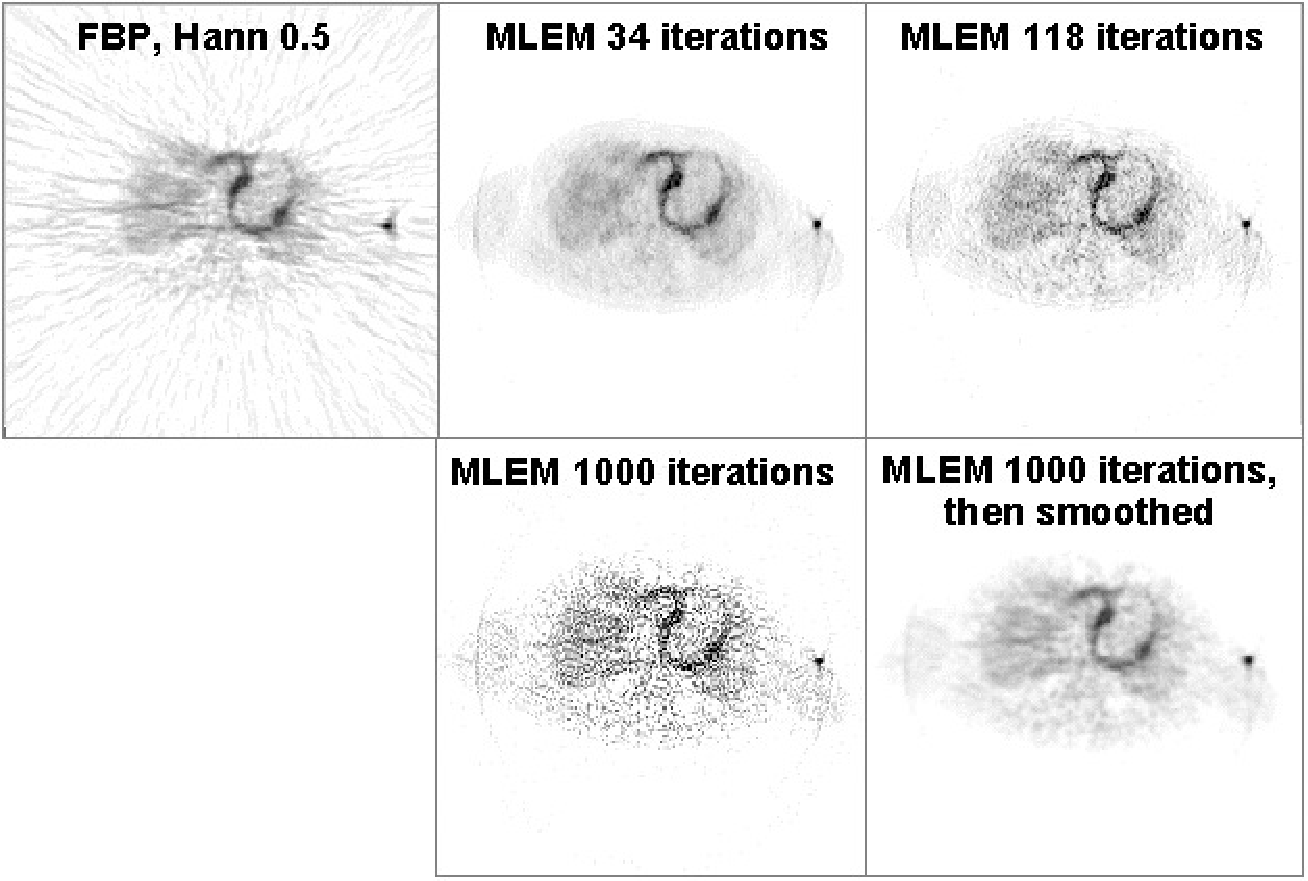
\includegraphics[width=0.9\textwidth]{figs/fig_mlem_1000iter.pdf}
\caption{\label{fig:mlem_1000iter} \emph{Reconstruction of a cardiac PET scan
with FBP, and with MLEM. The images obtained after 34, 118 and 1000 iterations
are shown. The image at 1000 iterations is very noisy, but a bit of smoothing
turns it into a very useful image.}}
\end{figure}
%
This is illustrated in figure \ref{fig:mlem_1000iter}. After 34 MLEM
iterations a ``nice'' image is obtained. After 1000 iterations, the image is
very noisy. However, this noise is highly correlated, and drops dramatically
after a bit of smoothing (here with a Gaussian convolution mask). 

From figures \ref{fig:mlem_converge} and \ref{fig:mlem_1000iter} it follows
that it is better to apply many iterations and remove the noise afterwards
with post-smoothing. In practice, ``many'' is at least 30 iterations for
typical SPECT and PET images, but for some applications it can mean several
hundreds of iterations. One finds that when more effects are included in
the reconstruction (such as attenuation, collimator blurring, scatter,
randoms...), more iterations are needed.  The number also depends on the image
size, more iterations are needed for larger images. So if computer time is not
a problem, it is recommended to apply really many iterations (several
hundreds) and regularize with a prior or with post-smoothing.

\subsection{OSEM} \label{sec:osem}
%==========================
\begin{figure}[tb]
\centering
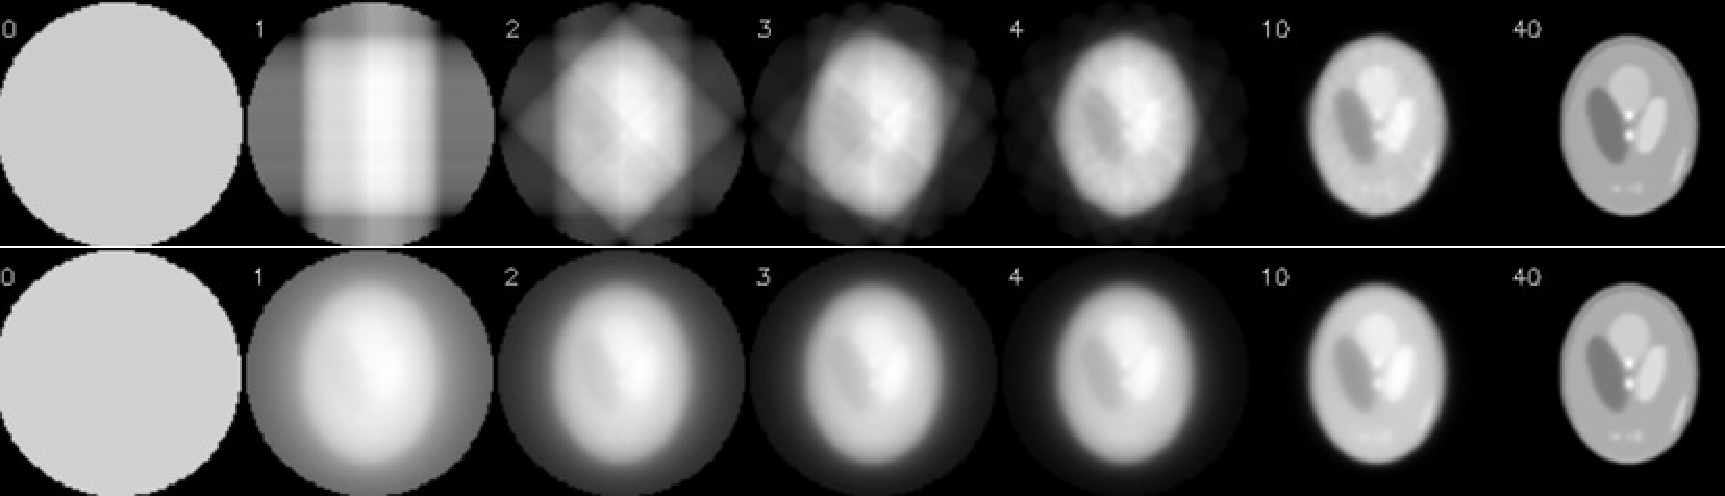
\includegraphics[width=\textwidth]{figs/fig_osem.pdf}
\caption{\label{fig:osem} \emph{Illustration of OSEM: there are 160
    projections in the sinogram, for an acquisition over
    360\textdegree. OSEM used 40 subsets of 4 projections each, the first
    subset has projections at 0\textdegree, 90\textdegree, 180\textdegree and
    270\textdegree. The second subset starts at 45\textdegree and so on. One
    OSEM iteration has 40 subiterations. The top row shows the first
    few and the last subiteration of OSEM. The bottom row shows the
    corresponding MLEM-iterations, where all projections are used for
    each iteration.}}
\end{figure}
In each iteration, MLEM must compute a projection and a
backprojection, which is very time consuming. FBP is much faster, it
uses only a single backprojection, the additional cpu-time for the
ramp filtering is small. Consequenly, the computation of 30 MLEM
iterations takes about 60 times longer than an FBP
reconstruction. MLEM was invented by Shepp and Vardi in 1982, but the
required cpu time prohibited application in clinical routine. Only
after 1992 clinical application started, partly because the computers
had become more powerful, and partly because a very simple
acceleration trick was proposed by Hudson and Larkin. The trick is
called ``ordered subsets expectation maximisation (OSEM)'', and the
basic idea is to use only a part of the projections in every
ML-iteration. This is illustrated in fig \ref{fig:osem}. In this
example, there are 160 projections, which are divided in 40 subsets of
4 projections per subset. The first subset contains the projections
acquired at 0\textdegree, 90\textdegree, 180\textdegree and 270\textdegree. The
second subset has the projections at 45\textdegree, 135\textdegree,
225\textdegree and 315\textdegree and so on. One OSEM iteration consists of
40 subiterations. In the first subiteration, the projection and
backprojection is restricted to the first subset, the second
subiteration only uses the second subset and so on. After the last
subiteration, all projections have been used once. As shown in fig
\ref{fig:osem}, 1 OSEM iteration with 40 subsets produces an image
very similar to that obtained with 40 MLEM iterations. Every MLEM
iteration uses all projections, so in this example, OSEM obtains the
same results 40 times faster.

A single OSEM iteration can be written as
\begin{equation}
  \lambda_j^{new}  =  \frac{\lambda_j^{old}}{\sum_{i\in S_k} c_{ij}}
           \sum_{i\in S_k} c_{ij}  \frac{q_i}{\sum_j c_{ij} \lambda_j^{old}},
           \label{eq:osem}
\end{equation}
where $S_k$ is subset $k$. Usually, one chooses the subsets such that
every projection is in exactly one subset.

The characteristics of OSEM have been carefully studied, both
theoretically and in practice. In the presence of noise, it does not
converge to a single solution, but to a so-called limit cycle. The
reason is that the noise in every subset is different and
``incompatible'' with the noise in the other subsets. As a result,
every subset asks for a (slightly) different solution, and in every
subiteration, the subset in use ``pulls'' the image towards its own
solution. More sophisticated algorithms with better or even guaranteed
convergence have been proposed, but because of its simplicity and good
performance in most cases, OSEM is now by far the most popular
ML-algorithm on SPECT and PET systems.



\section{Fully 3D Tomography}
%%%%%%%%%%%%%%%%%%%%%%%%%%%%%
Until now, we have only discussed the reconstruction of a single 2D slice from
a set of 1D projection data. An entire volume can be obtained by
reconstructing neighboring slices.  This is what happens in SPECT with
parallel hole or fan beam collimation, in 2D PET and in single slice CT.

In some configurations this approach is not possible and the problem
has to be treated as a fully three-dimensional one. There are many
different geometries of mechanical collimators, and some of these
acquire along lines that cannot be grouped in parallel sets. Examples
are the cone beam and pinhole collimators in SPECT (fig
\ref{fig:collimators}). Another example is 3D PET (section
\ref{sec:2D3DPET}). Three approaches to fully 3D reconstruction are
discussed below.

Note that the terminology may create some confusion about the
dimensions. 2D PET actually generates 3D sinogram data: the dimensions
are the detector and the projection angle (defining the projection
line within one slice), and the position of slice. Fully 3D PET
produces 4D sinogram data. The PET detector covers typically a
cylindrical surface. Two coordinates are needed to identify a single
detector, hence four coordinates are needed to identify a projection
line between a pair of detectors. And as will be discussed later, a series
of images can be acquired over time (dynamic acquisitions), which adds
another dimension to the data.


\subsubsection{Filtered backprojection}
%---------------------------------------
Filtered backprojection can be extended to the fully 3D PET case. The data are
backprojected along their detection lines, and then filtered to undo the
blurring effect of backprojection. This is only possible if the sequence of
projection and backprojection results in a shift-invariant point spread
function. And that is only true if every point in the reconstruction volume is
intersected by the same configuration of measured projection lines.

This is often not the case in practice. Points near the edge of the field of
view are intersected by fewer measured projection lines. In this case, the
data may be completed by computing the missing projections as follows. First a
subset of projections that meets the requirement is selected and reconstructed
to compute a first (relatively noisy) reconstruction image. Next, this
reconstruction is forward projected along the missing projection lines, to
compute the missing data. Then, the computed and measured data are combined
into a single set of data, that now meets the requirement of shift-invariance.
Finally, this completed data set is reconstructed with 3D filtered
backprojection.

\subsubsection{ML-EM reconstruction}
%-----------------------------------
ML-EM can be directly applied to the 3D data set: the formulation is very
general, the coefficients $c_{ij}$ in (\ref{eq:jnmlem}) can be directly used
to describe fully 3D projection lines.

In every iteration, we have to compute a projection and a backprojection along
every individual projection line. As a result, the computational burden may
become pretty heavy for a fully 3D configuration.


\subsubsection{Fourier rebinning}
%--------------------------------
In PET, a rebinning algorithm is an algorithm that resamples the data
in the sinogram space, so as to reorganize them into a form that
leads to a simpeler reconstruction.
%
In 1997, an exact rebinning algorithm, called {\em Fourier rebinning},
was derived. It converts a set of 3D data into a set of 2D
projections. Because all photons acquired in 3D are used to compute
the rebinned 2D data set, the noise in this data set is much lower
than in the corresponding 2D subset, which is a part of the original
3D data.

These projections can be reconstructed with standard 2D filtered
backprojection.  It was also shown that the Poisson nature of the data
is more or less preserved.  Consequently, the resulting 2D set can be
reconstructed successfully with the 2D ML-EM algorithm as
well. (Fourier rebinning is based on a wonderful feature of the
Fourier transform of the sinograms, hence its name.)

In practice, the exact rebinning algorithm is not used. Instead, one
only applies an approximate expression derived from it, because it is
much faster and sufficiently accurate for most configurations. This
algorithm (called FORE) is available on all commercial PET systems.

\section{Time-of-flight PET} \label{sec:TOF}
%%%%%%%%%%%%%%%%%%%%%%%%%%%%%
The speed of light is c = 30 cm/ns. Suppose that a point source is put
exactly in the center between two PET detectors, which are connected
to coincidence electronics. If two photons from the same annihilation
are detected, then they must have arrived simultaneously in the
respective detectors. However, the timing will be different if the
source is moved 15 cm towards one detector. The photon will arrive in
that detector 0.5 ns earlier, the other photon will arrive in the
other detector 0.5 ns later. Consequently, if the electronics can
measure the difference in arrival times $\Delta t$, then the position
of the annihilation along the projection line can be deduced: $\Delta
R = c \Delta t / 2$, where $\Delta R$ is the distance to the
center. Using this principle in PET is called time-of-flight PET or
TOF-PET.

In the eighties, TOF-PET scanners were built, but their performance
was disappointing. To obtain a reasonable TOF resolution, one needs to
measure the arrival time very accurately. Consequently, crystal
detectors with a very short scintillation time must be used. Such
crystals were available (e.g. CsF), but these fast crystals all had a
poor stopping power (low attenuation coefficient) at 511
keV. Consequently, the gain obtained from the TOF-principle was more
than offset by the loss due to the decreased detection
sensitivity. For that reason, TOF was abandoned, and nearly all
commercial PET scanners were built using BGO, which has a very high
stopping power but a long scintillation time (see table
\ref{tab:crystals}).

More recently, new scintillation crystals have been found, which
combine high stopping power with fast scintillation decay (table
\ref{tab:crystals}). In current scanners, LSO (or LYSO) is mostly
used. And since the eighties, the electronics have become faster as
well. The current commercial TOF-PET systems have a TOF resolution
ranging from around 500 ps (7.5 cm) for older systems to around 200 ps
for new systems (new in 2020).

\begin{figure}[t]
\centering
  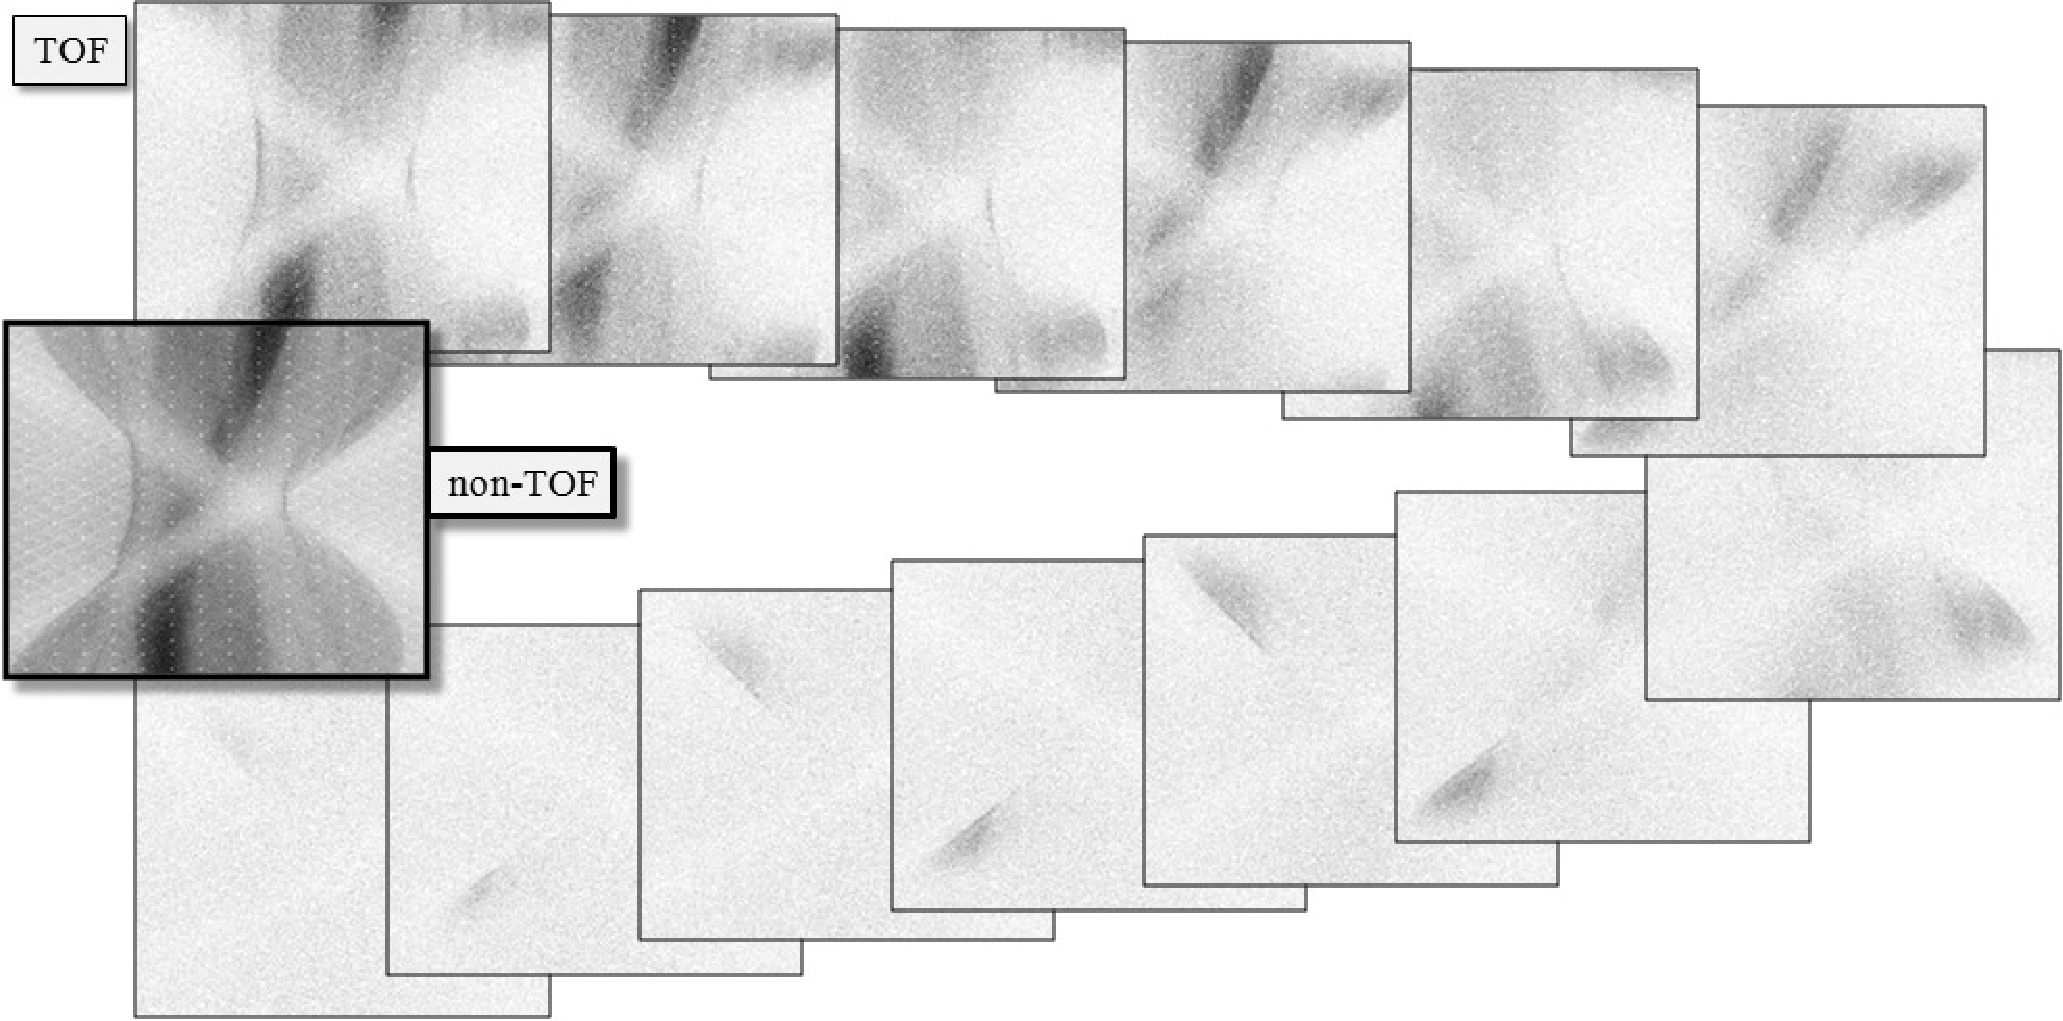
\includegraphics[width=0.72\textwidth]{figs/fig_tofsino.pdf}
  \vspace{-4mm}
  \caption{\label{fig:tofsino} \emph{A single plane from a clinical
  TOF-data set, sampled at 13 TOF-bins. The first bin corresponds to
  the center, the subsequent bins are for increasing distances,
  alternatedly in both directions. The non-TOF sinogram was obtained
  by summing the 13 TOF-sinograms.}}
\end{figure}
TOF-PET sinograms (or projections) have one dimension more than the
corresponding non-TOF data, because with TOF, the position along the
projection line is estimated as well. Figure \ref{fig:tofsino} shows a
TOF sinogram (sampled at 13 TOF-bins) together with the non-TOF
sinogram (obtained by adding all TOF-bins).

Consequently, a parallel projection of a 2D image along a single
projection angle, is not a 1D profile but a 2D image. This projection
can be considered as a blurred version of the original image, where
the blurring represents the uncertainty due to the point spread
function of the TOF-position measurement. This can be well modeled as
a 1D Gaussian blurring, as illustrated in fig \ref{fig:TOFproj}.
\begin{figure}[tb]
\centering
  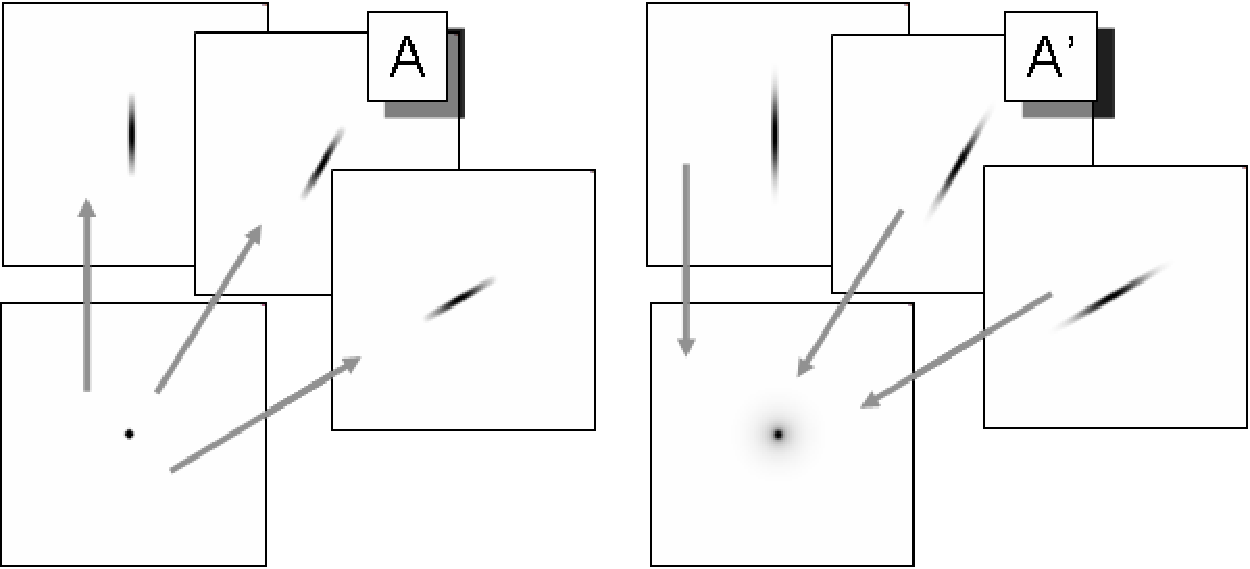
\includegraphics[width=0.7\textwidth]{figs/fig_TOF_projbproj.pdf}
  \caption{\label{fig:TOFproj} \emph{Left: TOF-PET projection (matrix
  A) can be considered as a 1D smoothing along the projection
  angle. Right: the TOF-PET backprojection of TOF-PET projection is
  equivalent to a 2D blurring filter. The blurring is much less than
  in the non-TOF case (fig \ref{fig:backproj}).}}
\end{figure}


For iterative reconstruction, one will need the corresponding
backprojection operator. Using the discrete representation, the
projection can be written as:
\begin{equation}
  q_i = \sum_j c_{ij} \lambda_j,
\end{equation}
which is the same expression as for non-TOF-PET and SPECT
(eq. \ref{jn:mlproj}), but of course, the elements $c_{ij}$ of the
system matrix are different. The corresponding backprojection is then
given by
\begin{equation}
  b_j = \sum_i c_{ij} q_i.
\end{equation}
The transpose of a symmetrical blurring operator is the same blurring
operator. Consequently, every TOF-projection image must be blurred
with its own 1D blurring kernel, and then they all have to be summed
to produce the backprojection image. The PSF of projection followed by
backprojection then yields a circularly symmetrical blob with central
profile
\begin{equation}
  b(r) = \mbox{Gauss}(r,\sqrt{2}\sigma) \frac{1}{|r|}, \label{eq:TOFpsf}
\end{equation}
where $r$ is the distance to the center of the blob, $\sigma$ is the
standard deviation of the Gaussian blurring that represents the TOF
resolution, and Gauss($r,s$) is a Gaussian with standard deviation
$s$, evaluated in $r$. The standard deviation in (\ref{eq:TOFpsf}) is
$\sqrt{2}\sigma$ and not simply $\sigma$, because the blurring has
been applied twice, once during projection and once during
backprojection. See appendix \ref{app:bprojproj} for a more
mathematical derivation.

For very large $\sigma$, this reduces to $b(r) = 1 / |r|$, which is
the result for backprojection in non-TOF PET, obtained just after eq
(\ref{eq:bprojvalue}). The projection and backprojection operators
are illustrated in fig \ref{fig:TOFproj}.

Also for TOF-PET, filtered backprojection algorithms can be
developed. Because of the data redundancy, different versions of FBP
can be derived. A natural choice is to use the same backprojector as
mentioned above. With this backprojector, the backprojection of the
TOF-PET measurement of a point source will yield the image of blob
given by eq (\ref{eq:TOFpsf}). Consequently, the reconstruction filter
can be obtained by computing the inverse operator of
(\ref{eq:TOFpsf}). As before, the filter can be applied before
backprojection (in the sinogram) or after backprojection (in the
image), because of the Fourier theorem.

\begin{figure}[tb]
\centering
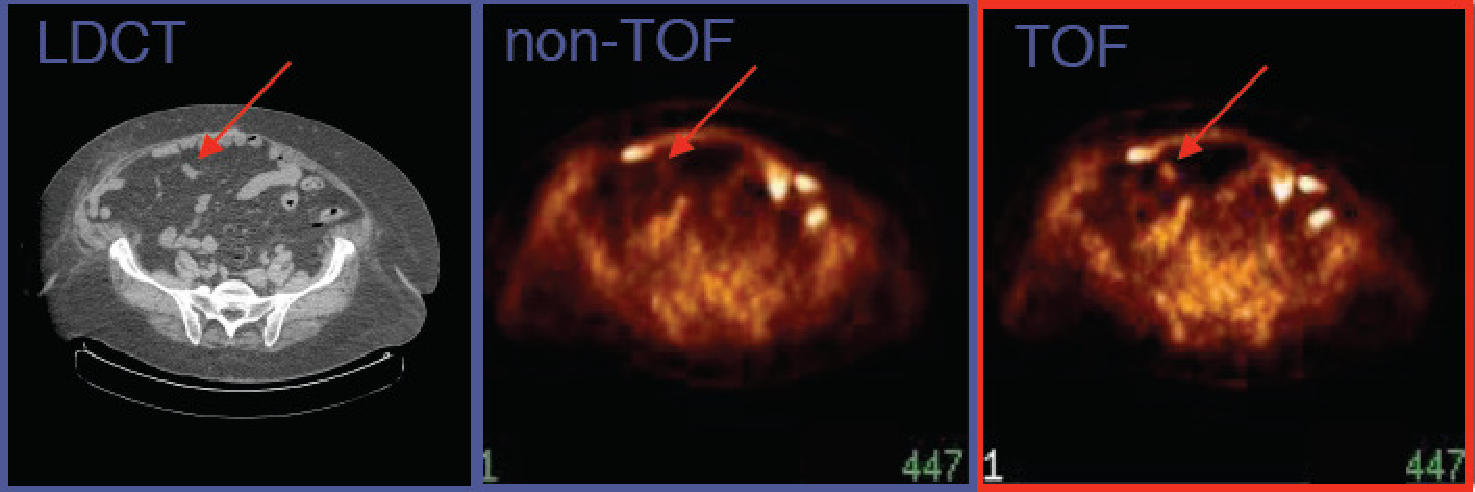
\includegraphics[width=0.9\textwidth]{figs/fig_TOF_matej.pdf}
\caption{\label{fig:TOFmatej} \emph{CT and TOF-PET image, acquired on
    a PET/CT system with time-of-flight resolution of about 700
    ps. The TOF-PET image reveals a small lesion not seen on the
    non-TOF PET image. (Courtesy Joel Karp and Samuel Matej,
    University of Pennsylvania. The image is acquired on a Philips
    Gemini TOF-PET system)}}
\end{figure}

Figure \ref{fig:TOFmatej} compares a TOF and non-TOF image. By
discarding the TOF-information, TOF-PET data can be converted to
regular PET data. This was done here to illustrate the improvement
obtained by using TOF. There are several reasons why the TOF-PET image
is better.

First, because more information is used during reconstruction, the
noise propagation is reduced, resulting in a better signal-to-noise
ratio (less noise for the same resolution) in the TOF image. It has
been shown that, for the center of a uniform cylinder, improving the
TOF resolution with a factor reduces the variance in the reconstructed
image with that same factor, at least if these images have the same
spatial resolution.

Second, it turns out that the convergence of the MLEM algorithm is
considerably faster for TOF-PET. It is known that MLEM converges
faster for smaller images, because the correct reconstruction of a
pixel depends on the reconstruction of all other pixels that share
some projection lines with it. The TOF information reduces that number
of information-sharing pixels considerably. Because in clinical
routine, usually a relatively low number of iterations is applied,
small image detail (high spatial frequencies) may suffer from
incomplete convergence. It was found that after introducing TOF, the
spatial resolution of the clinical images was better than before. TOF
has no direct effect on the spatial resolution, but for a similar
number of iterations, MLEM converges faster, producing a better
resolution. And because of the improved SNR, it can achieve this
better resolution at a similar or better noise level than non-TOF
PET. 

Third, an additional advantage of this reduced dependency on other
pixels is a reduced sensitivity to most things that may cause
artifacts, such as errors in the attenuation map, patient motion, data
truncation and so on. In non-TOF PET, the resulting artifacts can
propagate through the entire image. In TOF-PET, that propagation is
reduced because of the reduced dependencies between the reconstructed
pixel values.

Finally, the gain due to TOF is higher when the region of interest is
surrounded by more activity and if the active object (i.e. the patient
body) is larger. The reason is that in those cases, there is more to
be gained by suppressing sensitivity to surrounding activity, since
there is more surrounding activity. As a result, TOF helps more in
situations where non-TOF MLEM performs poorest. The opposite is also
true, for imaging a point source, TOF-PET does not better than non-TOF
PET.

%%%%%%%%%%%%%%%%%%%%%%%%%%%%%
\section{Reconstruction with resolution modeling} \label{sec:resol}
%%%%%%%%%%%%%%%%%%%%%%%%%%%%%
In every MLEM iteration a projection and backprojection is
executed. The projection $\sum_j c_{ij} \lambda_j$ simulates the
acquisition and the backprojection $\sum_i c_{ij} q_i$ is the
corresponding adjoint operator. A more accurate simulation of the
acquisition should result in a more accurate reconstruction of the
image from the acquired tomographic data. In SPECT, the system matrix
elements $c_{ij}$ should account for the position dependent
attenuation to ensure that MLEM produces quantitative images. In PET,
the elements $c_{ij}$ should model the attenuation and detector
sensitivities (see equation \ref{eq:petnorm}), and for TOF-PET, also
the width of the TOF-resolution.

\begin{figure}[htb]
\centering
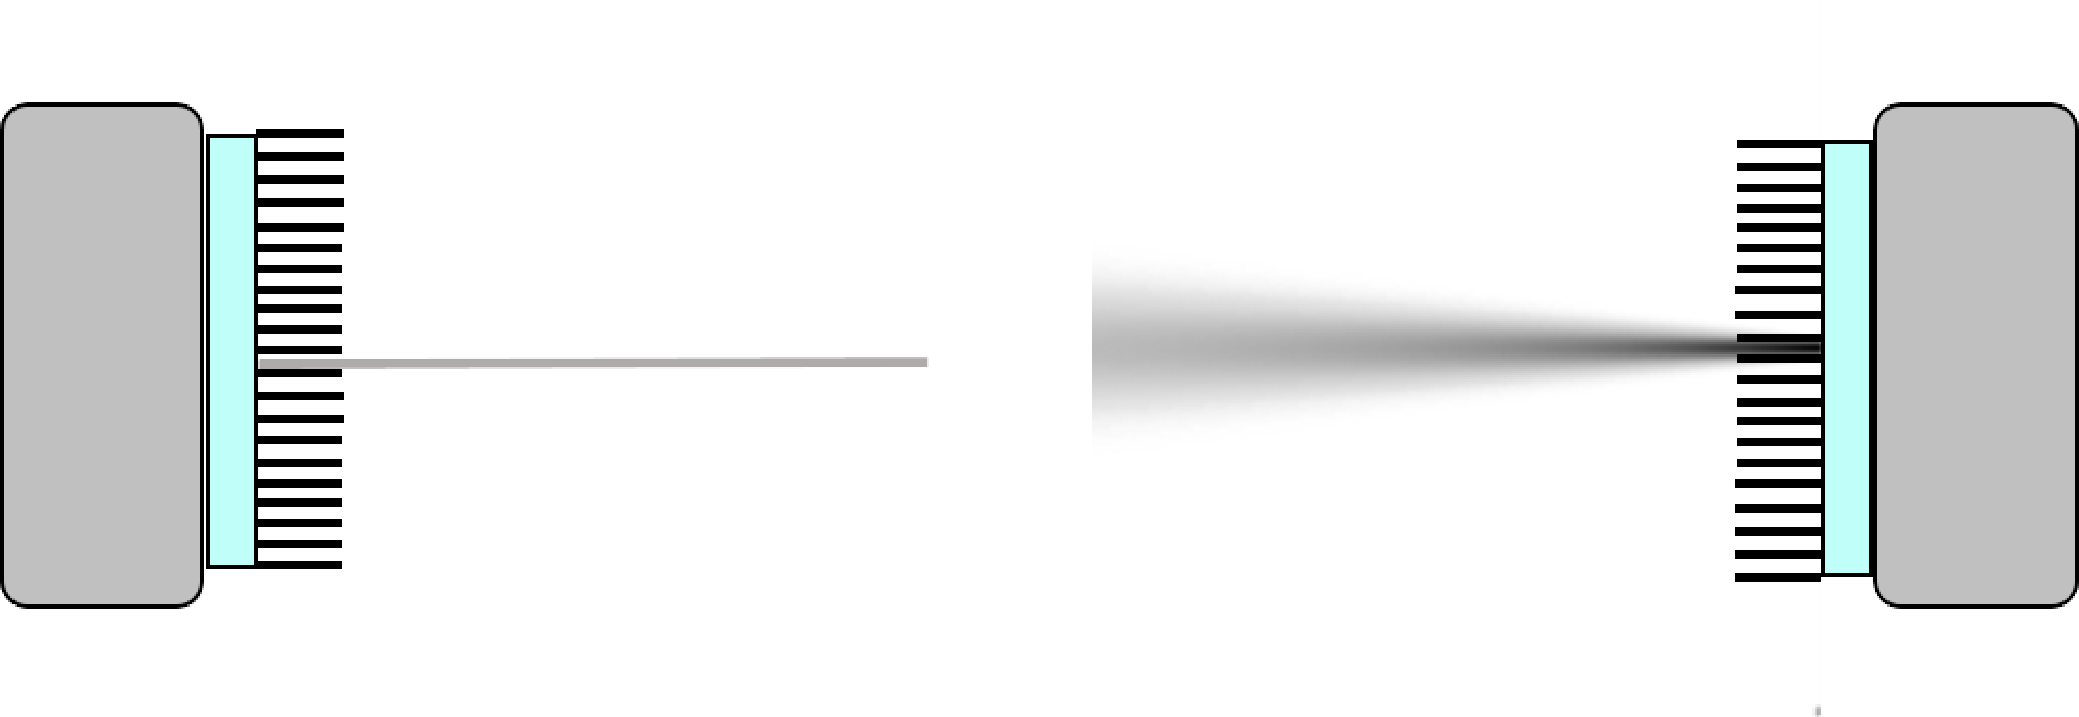
\includegraphics[width=0.9\textwidth]{figs/fig_resol_line_cone.pdf}
\caption{\label{fig:resolcone} \emph{In a simple projector/backprojector,
    the projection is modeled as a (weighted) line integral. To
    account for the position dependent collimator blurring, the line
    integral can be replaced by a weighted integral over a cone.}}
\end{figure}
In section \ref{sec:collimation}, we have seen that gamma cameras
suffer from position dependent collimator blurring. As illustrated in
figure \ref{fig:resolcone}, this can be modeled by computing the
projection not as a line integral, but as the integral over a cone,
using appropriate weights to model the position dependent PSF. This
position dependent blurring is then combined with the attenuation to
obtain the system matrix elements $c_{ij}$. The same can be done for
PET: the blurring due to the detector width (and if desired, also the
positron range and/or the acolinearity) can be incorporated in the PET
or TOF-PET system matrix elements.

During the iterations, MLEM (or OSEM) uses the system matrix in every
projection and backprojection, and by doing so, it will attempt to
invert all effects modeled by that system matrix. If the system matrix
models a blurring effect, then MLEM will automatically attempt to undo
that blurring. This produces images with improved resolution as
illustrated for a SPECT and a PET case in figure
\ref{fig:resolspectpet}. Interestingly, modeling the finite system
resolution in MLEM not only improves the resolution in the
reconstructed image, it also suppresses the noise, as can be seen in
the PET reconstruction.

\begin{figure}[htb]
\centering
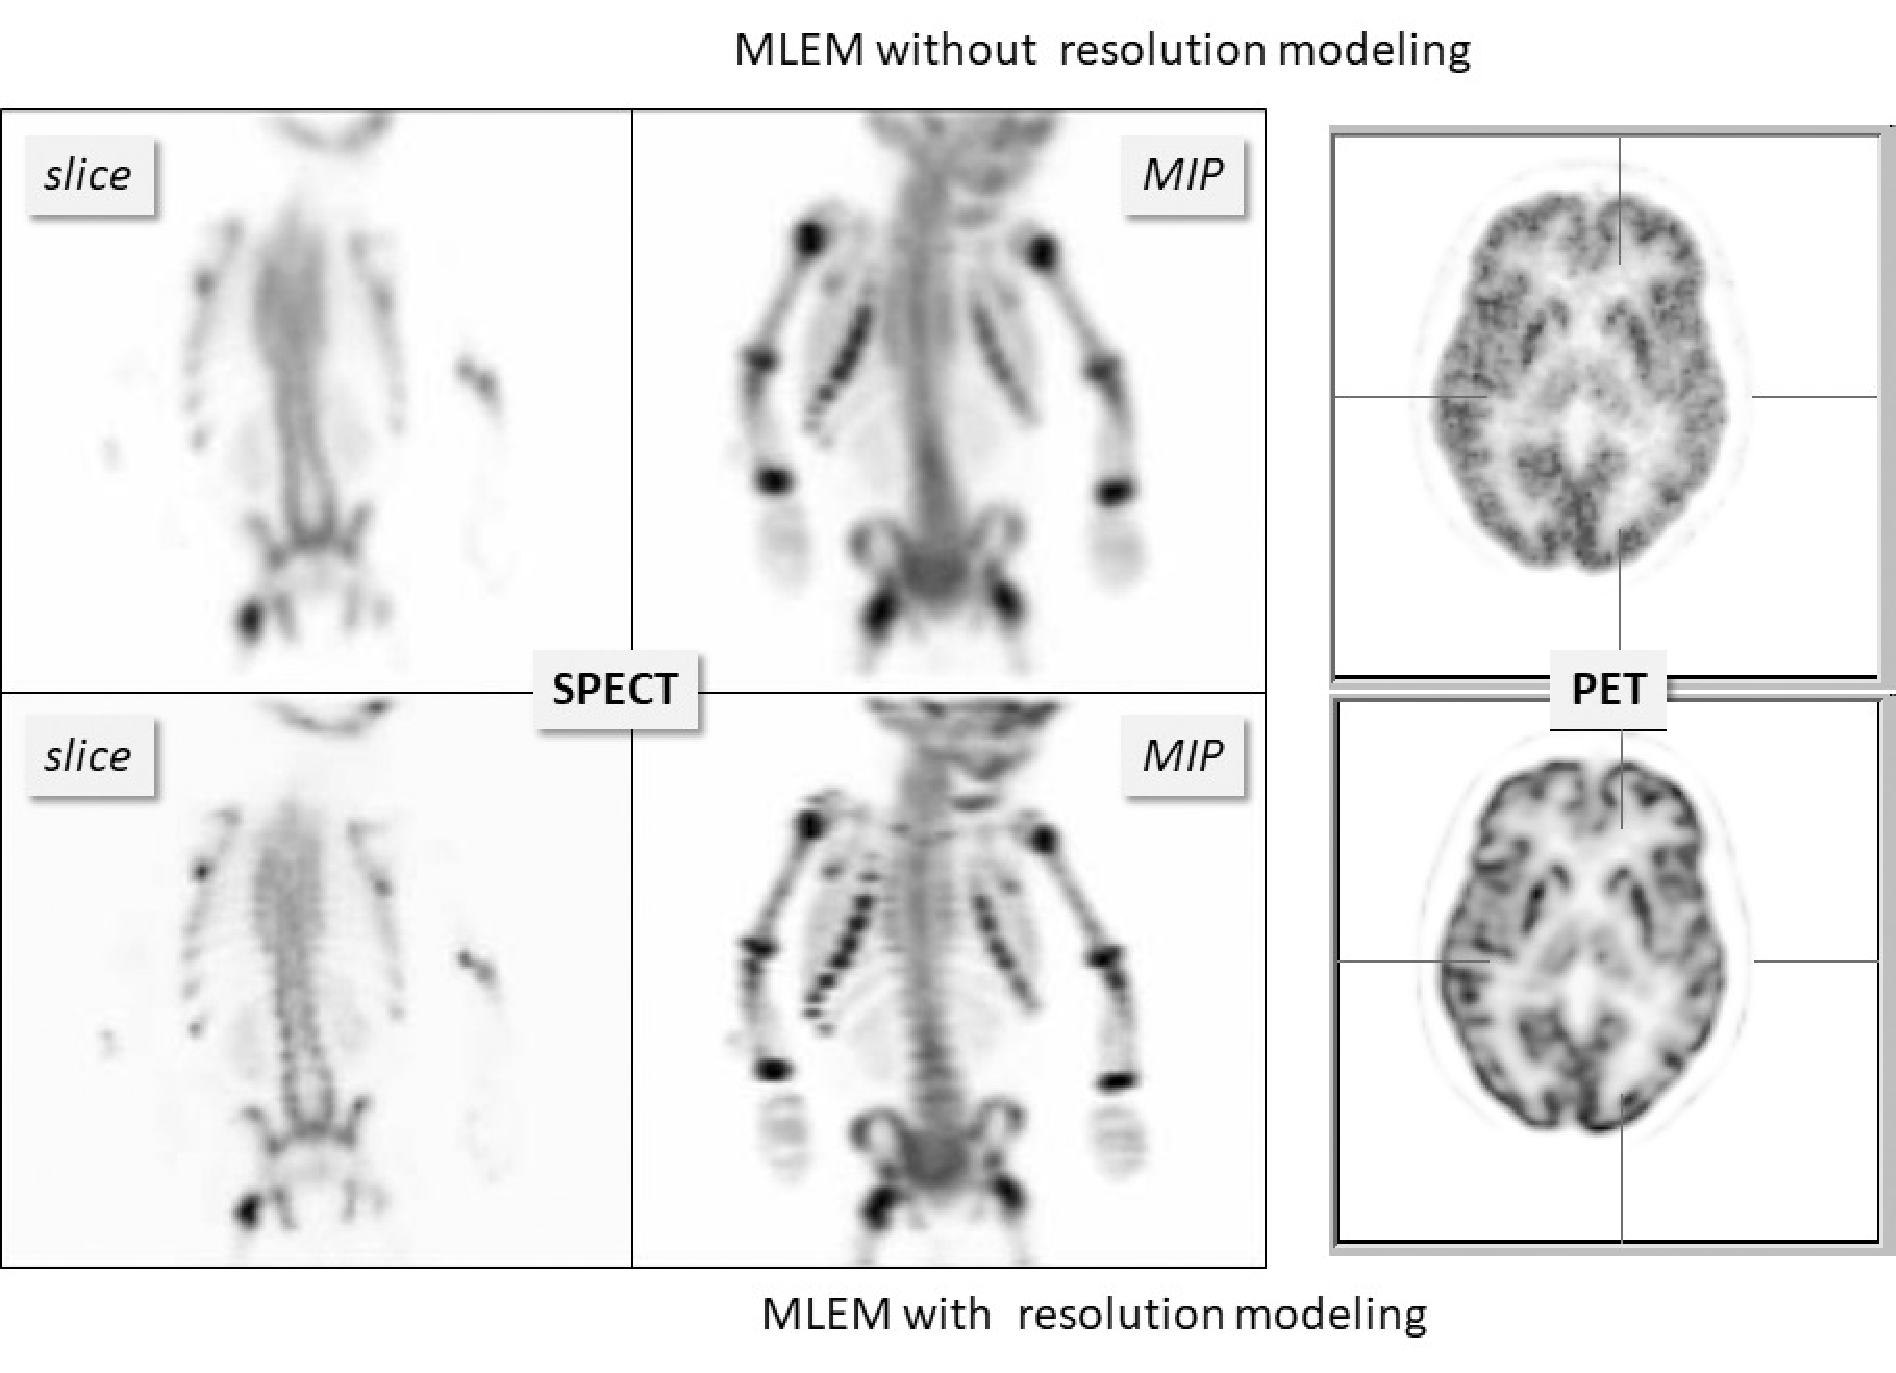
\includegraphics[width=0.9\textwidth]{figs/fig_resol_spectpet.pdf}
\caption{\label{fig:resolspectpet} \emph{Reconstructions with and
    without resolution modeling from a SPECT bone scan of a child and
    a brain PET scan. ``MIP'' denotes ``maximum intensity
    projection''.  MLEM with resolution modeling recovers image detail
    that was suppressed by the finite system resolution.}}
\end{figure}

However, the deblurring cannot be 100\% successful, because deblurring
is a very ill-posed problem. Except in special cases, deblurring
problems have multiple solutions, and iterative algorithms cannot
``know'' which of those possible solutions they should produce. This
is illustrated in figure \ref{fig:resolpetgibbs}. A noise-free PET
simulation was done, accounting for finite spatial resolution. MLEM
images without and with resolution modeling were reconstructed from
the noise-free sinogram. The figure shows that MLEM with resolution
modeling produced a sharper image, but that image is different from
the true image that was used in the simulation. 
\begin{figure}[htb]
\centering
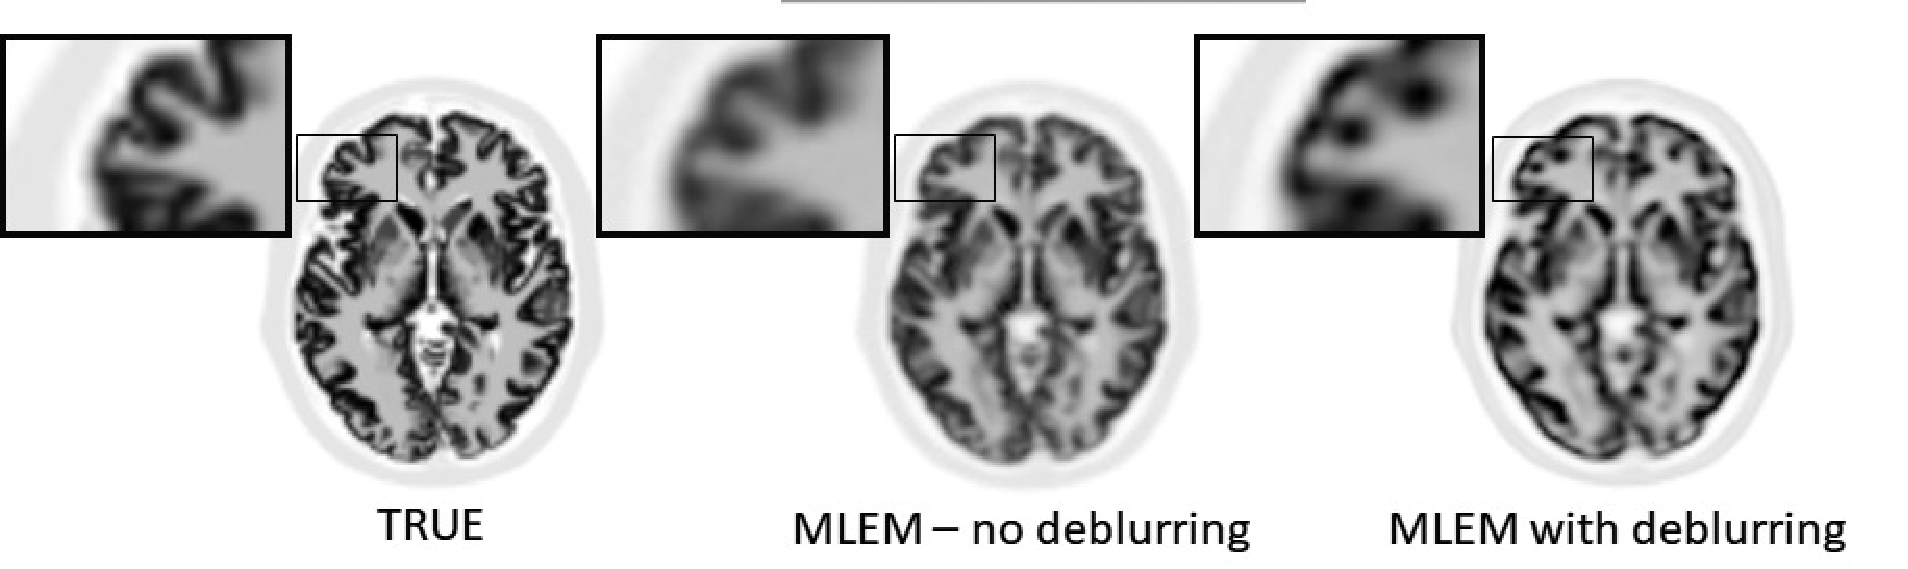
\includegraphics[width=0.9\textwidth]{figs/fig_resol_petgibbs.pdf}
\caption{\label{fig:resolpetgibbs} \emph{PET simulation without noise
    but with finite resolution modeling. MLEM with deblurring produced
    sharper images, but they are clearly different from the ground truth.}}
\end{figure}

The problem is that the blurring during the projection not only
suppresses some information, it also erases some information. MLEM can
recover image details that have been suppressed but are still present
in the data, but no algorithm can recover details that have been
erased from the data. This can be best explained in the frequency
domain.

Figure \ref{fig:resolgibbs} shows a simple 1D thought experiment. In
this experiment, we consider the PSF and its frequency spectrum. The
frequency spectrum of the PSF is often called the modulation transfer
function (MTF), because it tells us how the PSF of a system affects
(modulates) all frequency components of a signal which is transferred
through that system. Assume we are doing measurements on something
that can be well represented by a 1D profile. The true profile has a
single non-zero element. A measurement of that profile produces a
blurred version of the true profile. We assume that the measurement
device has a Gaussian PSF. The Fourier transform of a Gaussian is a
Gaussian, so the Gaussian PSF corresponds to a Gaussian MTF; denoting
the Fourier transform with ${\cal F}$, we have:
\begin{equation}
  {\cal F} \left( \frac{1}{\sqrt{2 \pi} \sigma}
     e^{-\frac{x^2}{2\sigma^2}} \right)
  = e^{- 2 \pi^2 \sigma^2 f^2}.
\end{equation}
The wider the Gaussian PSF, the narrower the corresponding Gaussian
MTF, and the larger the fraction of frequencies that are suppressed so
much that they will be lost in the noise.
%
\begin{figure}[htb]
\centering
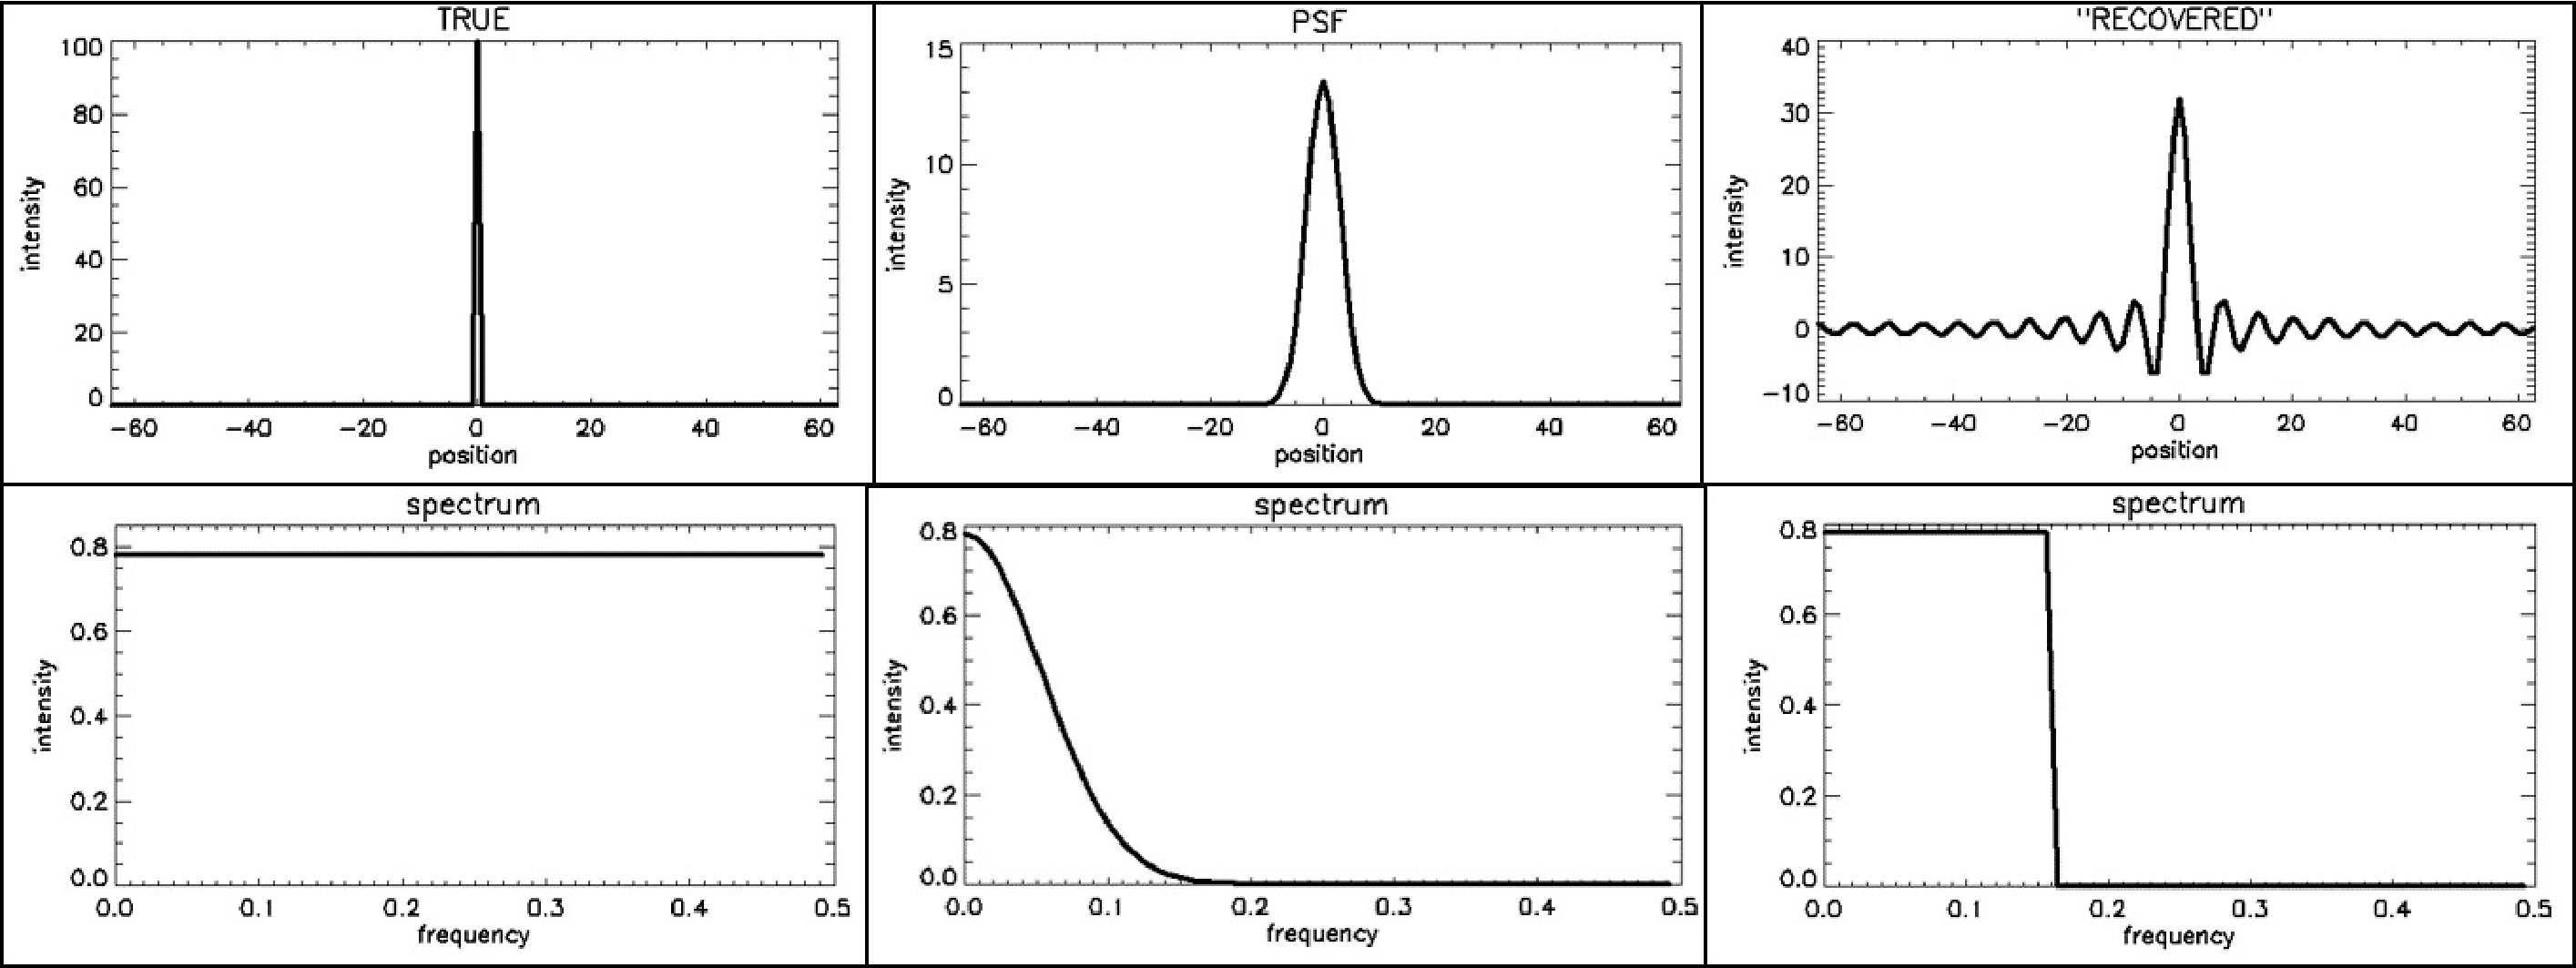
\includegraphics[width=0.9\textwidth]{figs/fig_resol_gibbs.pdf}
\caption{\label{fig:resolgibbs} \emph{Impulse responses (top) and
    their corresponding frequency spectra or MTF (bottom). From left
    to right: (1) the ideal PSF (a flat MTF), a Gaussian PSF (Gaussian
    MTF) and a sinc-shaped PSF, corresponding to a rectangular MTF}}
\end{figure}
%
Now imagine that we apply some deblurring algorithm, which restores
the frequency components that are still present in the data. We also
assume that it does not ``invent'' data, but assumes that things not
seen by the measurement should be set to zero. That will result in an
approximately rectangular PSF. This is illustrated in figure
\ref{fig:resolgibbs}, where we assumed that all frequencies below 0.16
could still be restored, whereas the higher frequencies were filtered
away by the measurement PSF. The inverse Fourier transform of a
rectangular function is a sinc function ($\mbox{sinc}(x) =
\sin(x)/x$), as can easily be verified:
\begin{align}
  {\cal F}^{-1}(\mbox{rectangle}_{f_c}(f))
  &= \int_{-\infty}^{\infty} \mbox{rectangle}_{f_c}(f) e^{2j\pi f x}
  df \nonumber\\
  &= \int_{-f_x}^{f_c} e^{2j\pi f x} df \nonumber\\
  &= \frac{e^{2j\pi f_c x} - e^{- 2j\pi f_c x}}{2j\pi x} \nonumber\\
  &= \frac{2j \sin(2\pi f_c x)}{2j\pi x} \nonumber\\
  &= \frac{\sin(2\pi f_c x)}{ \pi x},
\end{align}
where we used $e^{jx} = \cos(x) + j \sin(x)$, and $j =
\sqrt{-1}$. Figure \ref{fig:resolgibbs} shows a sinc function (to plot
the function, make us of $\lim_{x \rightarrow 0} \sin(x)/x = 1$). The PSF
will oscillate at the cutoff frequency, so the wider the rectangular
MTF, the narrower the central peak of the PSF and the narrower the
ripples surrounding it.

Knowing the PSF, we can compute what the deblurred measurement will
look like for any other signal, by convolving that signal with the
PSF. Figure \ref{fig:resolsinc} shows the result for a block-shaped
signal. The result is still block-like, but the two edges are less
steep and are accompanied by ripples creating under- and
overshoots. These ripples are often called Gibbs artefacts.

\begin{figure}[htb]
\centering
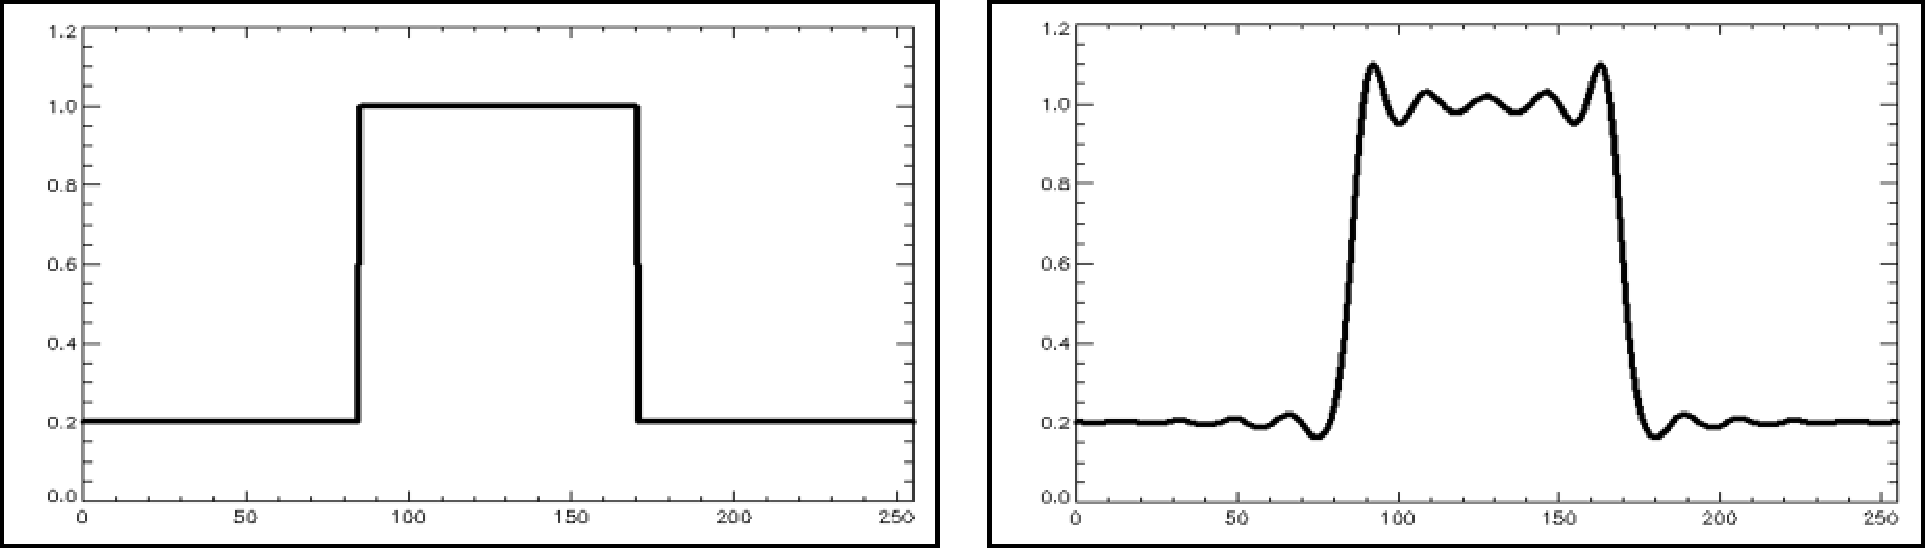
\includegraphics[width=0.9\textwidth]{figs/fig_resol_sinc.pdf}
\caption{\label{fig:resolsinc} \emph{The convolution of a block-shaped
    signal with a sinc-shaped PSF produces a smoother version of the
    block with ripples, also called Gibbs artefacts, on top of it.}}
\end{figure}

MLEM with resolution modeling combines reconstruction with deblurring
for the system PSF, which is more complicated than simple
deblurring. Nevertheless, when the system PSF is modeled during MLEM,
very similar Gibbs artefacts are created, because MLEM cannot restore
the higher frequencies that were lost due to that PSF. Because now the
blurring and deblurring are done in three dimensions, the Gibbs
artefact are rippling in 3D too. The effects in different dimensions
can accumulate, and as a result, the over- and undershoots can become
very large. E.g. for small hot objects, the overshoot can go as high
as 100\%. That is unfortunate, such high overshoots can cause problems
for quantitative analysis of the tracer uptake in small hot lesions,
as is often done in PET for oncology. Therefore, depending on the
imaging task, it may be necessary to smooth the image a bit to avoid
quantification errors due to these Gibbs effects.